% vim:tw=100:ts=4:sw=4:sts=4:et:
\section*{Vorlesung am 14.04.2011}

\begin{quote}
    It is quite natural that, after a lapse of about 2250 years, some details are now seen to be
    capable of improvement. (Coxeter, \cite[Section 1.2]{coxeter-1969})
\end{quote}

\subsection*{Hilbert}

\begin{itemize}
    \item In seinem Buch \cite{hilbert} hat David Hilbert (1862--1943) das Axiomensystem von Euklid
        gründlich überarbeitet.

    \item Hilbert verfolgt damit das Ziel, die Axiomatische Geometrie frei von unserer (oft in die
        Irre führenden) geometrischen Anschauung zu machen.

    \item Wir folgen im Wesentlichen der Aufarbeitung~\cite{hartshorne-2000} durch Robin Hartshorne
\end{itemize}

% BEM (taken from Wikipedia, http://en.wikipedia.org/wiki/Hilbert%27s_axioms): Other well-known
% modern axiomatizations of Euclidean geometry are those of Alfred Tarski and of George Birkhoff.

% ETWAS FORMALER:
% Formal "richtig" wäre es eine Menge von Punkten $\P$ einzuführen und eine Menge von Geraden $\MG$
% von Teilmengen von $\P$ (also \MG\subseteq 2^{\P}$. Eine Ebene~$\E$ ist dann ein Tripel $(\P,\MG,
% \MI)$ mit einer Inzidenzrelation $\MI$, die die Axiome I1,I2,I3 erfüllt.

Wir gehen aus von einer nichtleeren Menge~$\E$, deren Elementen wir {\em Punkte} nennen.
(Bezeichnung: $A,\,B,\,C,\ldots$).

{\em Geraden} sind gewisse Teilmengen von $\E$ (Bezeichnung: $g,\,h,\ldots$);

Man beachte, dass wir nicht erklären (können!) "`was Punkte und Geraden sind"'. Wir können aber
durch Axiome angeben welche Eigenschaften Punkte und Geraden haben oder wie sie zueinander in
Beziehung stehen.

% Wir betrachten 5 Gruppen von Axiomen:
% \begin{enumerate}
%     \item[I.] Axiome der Inzidenz
%     \item[II.] Axiome der Anordnung
%     \item[III.] Axiome der Kongruenz
%     \item[IV.] Axiome der Stetigkeit
%     \item[V.] Parallelenaxiom
% \end{enumerate}
% Die Axiome der Axiomengruppen I-IV sind die Axiome der
% "`{}absoluten
% Geometrie"'{}.\\

\subsection*{Inzidenzaxiome}

Wir sagen ein Punkt $A$ {\em inzidiert} mit einer Geraden $g$ genau dann wenn $A$ "`auf $g$ liegt"'
(bzw. $A\in g$).

\begin{itemize}
    \item[{\bf (I1)}] Zu je zwei verschiedenen Punkten $A,\,B\in\E$ gibt es genau eine Gerade
        $g\subset\E$ mit $A,\,B\in g$

    \item[{\bf (I2)}] Auf jeder Geraden gibt es mindestens 2 Punkte.

    \item[{\bf (I3)}] Es gibt 3 Punkte $A,\,B,\,C\in\E$, die nicht auf einer Geraden liegen
\end{itemize}

Die Gerade durch $A$ und $B$ in {\bf(I1)} bezeichnen wir auch mit $g(A,B)$. Drei Punkte $A,\,B,\,C$
heißen \emph{kollinear} wenn sie auf einer gemeinsamen Gerade liegen.  Das Axiom {\bf(I3)} sagt also
aus, dass es 3 nicht kollineare Punkte in $\E$ gibt.

Die Axiome sind {\em unabhängig voneinander}, d.h. eines kann nicht aus den anderen hergeleitet
werden. Für den Beweis der Unabhängigkeit betrachtet man Modelle (Beispiele), in denen alle Axiome
bis auf eins erfüllt sind.

\begin{center}
    % Vorlage:
    %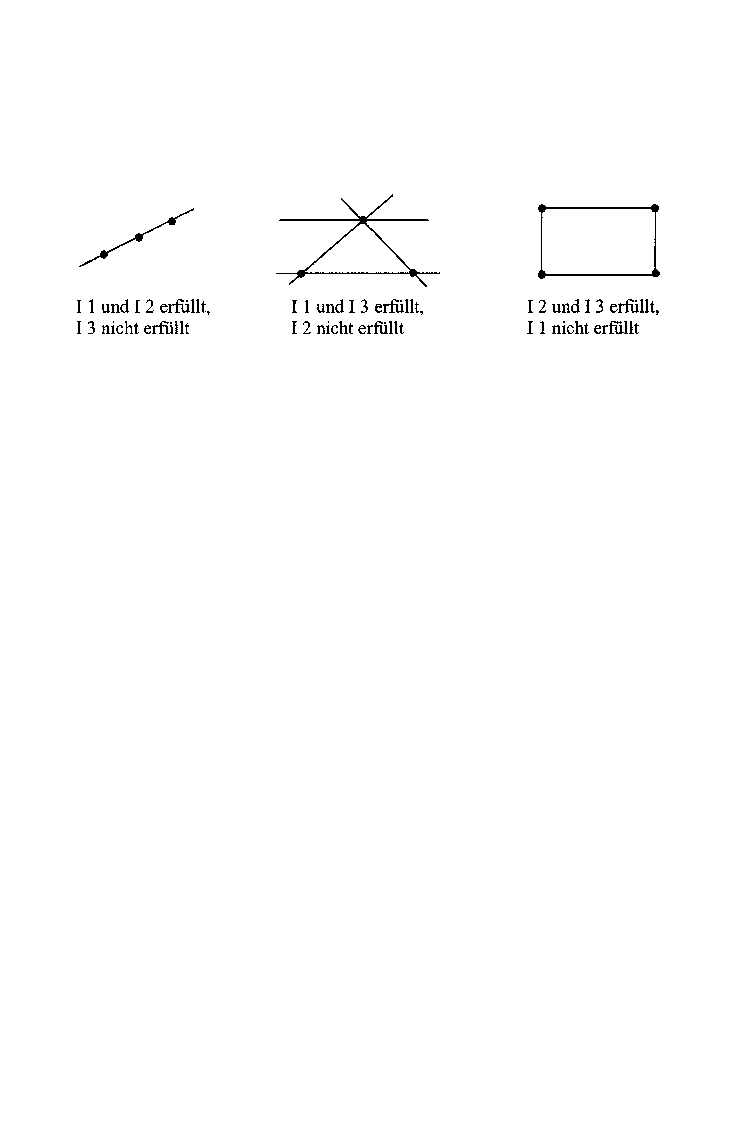
\includegraphics[width=12cm]{BILDER/BildUnabhaengigkeitInzidenzaxiome.pdf}

    % In den .tikz Dateien sind die Zeichnungen für die Bilder. Durch die Tabelle sieht der Abstand
    % zwischen den Bildern schöner aus.
    \begin{figure}[h]
        \begin{tabular}{ccc}
        \begin{tikzpicture}
	\fill [color=colPkt] (0,0) circle (1.5pt);
	\fill [color=colPkt] (1,0.5) circle (1.5pt);
	\fill [color=colPkt] (2,1) circle (1.5pt);
	\draw (-0.5,-0.25) -- (2.5,1.25);
	\draw (1,-0.5) node[anchor=north, text width=3.5cm] {(I1) und (I2) erfüllt, (I3) nicht erfüllt};
\end{tikzpicture}

        &
        \begin{tikzpicture}
	\fill [color=colPkt] (0,0) circle (1.5pt);
	\fill [color=colPkt] (2,0) circle (1.5pt);
	\fill [color=colPkt] (1,1) circle (1.5pt);
	\draw (-0.25,-0.25) -- (1.25,1.25);
	\draw (0.75,1.25) -- (2.25,-0.25);
	\draw (-0.35,0) -- (2.35,0);
	\draw (-0.35,1) -- (2.35,1);
	\draw (1,-0.5) node[anchor=north, text width=3.5cm] {(I1) und (I3) erfüllt, (I2) nicht erfüllt};
\end{tikzpicture}

        &
        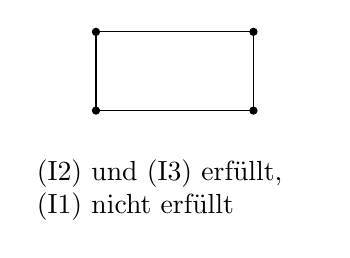
\begin{tikzpicture}
	\fill [color=black] (0,0) circle (1.5pt);
	\fill [color=black] (2,0) circle (1.5pt);
	\fill [color=black] (0,1) circle (1.5pt);
	\fill [color=black] (2,1) circle (1.5pt);
	\draw (0,0) -- (2,0) -- (2,1) -- (0,1) -- (0,0);
	\draw (1,-0.5) node[anchor=north, text width=3.5cm] {(I2) und (I3) erfüllt, (I1) nicht erfüllt};
\end{tikzpicture}

        \end{tabular}
        \caption{Unabhängigkeit der Inzidenzaxiome}
    \end{figure}
\end{center}

Eine Menge $\E$ von Punkten, mit einer Menge %$\MG$
von Geraden, die zusammen die Axiome {\bf(I1)}, {\bf(I2)} und {\bf(I3)} erfüllen, heißt auch {\em
Inzidenzgeometrie}. Wir bezeichnen $\E$ in diesem Fall auch als {\em Ebene}.
%Formal ist dies ein Tripel (\E,\MG,\MI) mit
%einer Inzidenzrelation $\MI\subseteq \E |times \MG$.
Auch wenn wir noch nicht viel gefordert haben, lassen sich schon erste einfache Schlußfolgerungen
ziehen, die für alle Inzidenzgeometrien gelten:

\begin{thm}
    Für eine Ebene $\E$, in der die Axiome {\bf(I1)}, {\bf(I2)} und {\bf(I3)} erfüllt sind, gilt:
    \begin{enumerate}
        \item Es gibt mindestens 3 paarweise verschiedene Geraden.

        \item Zwei verschiedene Geraden können höchsten einen gemeinsamen Punkte enthalten.
    \end{enumerate}
\end{thm}

\begin{proof}
    \begin{enumerate}
    \item[(2)] Enthalten zwei unterschiedliche Geraden $g$ und $h$ zwei unterschiedliche
        Schnittpunkte $A$ und $B$, so widerspricht das Axiom {\bf(I1)}, in der die Eindeutigkeit der
        Geraden durch $A$ und $B$ gefordert wird.

    \item[(1)] Nach Axiom {\bf(I3)} gibt es drei Punkte die nicht kollinear sind. Die Geraden
        $g(A,B), g(A,C)$ und $g(B,C)$ sind wiederum paarweise verschieden nach {\bf(I1)}.
    \end{enumerate}
\end{proof}

Man beachte, dass die Argumentation im Beweis unabhängig von unserer "`geometrischen Anschauung"'
ist. Wir können sogar {\em Modelle} angeben, die weit entfernt sind von unserer geometrischen
Anschauung einer Ebene, die aber trotzdem die Inzidenzaxiome erfüllen. Wir betrachten ein paar
Beispiele:

\begin{description}
    \item[Modell 1] $\E=\{A,\,B,\,C\}$ - 3 paarweise verschiedene Punkte;\\
        Geraden: mögliche Tupel $\{A,\,B\},\;\{A,\,C\},\;\{B,\,C\}$
        % Das kleinstmögliche Modell

    \item[Modell 2] \label{Modell2} $\E=\{A,\,B,\,C,\,D\}$ - 4 paarweise verschiedene Punkte;\\
        Geraden: mögliche Tupel $\{A,\,B\},\; \{A,\,C\},\; \{A,\,D\},\; \{B,\,C\},\; \{B,\,D\},\;
        \{C,\,D\}$
        % Das kleinst mögliche Modell einer affinen Inzidenzgeometrie
\end{description}

Ist $\E$ endlich so spricht man auch von einer {\em endlichen Geometrie}.  Solche Geometrien werden
in der {\em Kombinatorik} untersucht.

\begin{description}
    \item[Modell 3] $\E=\R^2$ und Geraden "`wie üblich"' als Lösungen linearer Gleichungen
        $a x + b y = c$ mit $a,b,c\in \R$ ($a,b$ nicht beide $0$).
        % Hier als Beispiel auch über anderen Körpern?!
        % Dann ist Modell 2 Spezialfall für $K=F_2$!

    \item[Modell 4] ("`Bierdeckelgeometrie"')\\ % nach Felix Klein
        $\E=\{ (x,y)\in\R^2 | x^2+y^2<1 \}$; Geraden sind die Geraden aus Modell 3 geschnitten mit
        $\E$

    \item[Modell 5] ("`Halbebenenmodell von Poincaré"')\\
        $\E=\{ (x,y)\in\R^2 | y>0 \}$; Geraden sind entweder Halbkreise oberhalb der $x$-Achse oder
        Halbgeraden Senkrecht zur $x$-Achse. Das rechte Bild zeigt wie die Gerade zu zwei
        verschiedenen Punkten konstruiert wird.

    \item[Modell 6] ("`Sphärisches Modell der projektiven Ebene"')\\
        $\E=\{ (x,-x)\in\R^{3+3} \ | \ x_1^2+  x_2^2 + x_3^2= 1 \}$, d.h., Punkte sind in diesem
        Modell Paare von diametral liegenden Vektoren auf der Einheitssphäre; Geraden sind
        Punktmengen die auf einem Großkreis (Schnitt der Sphäre mit einer $2$-dimensionalen Ebene
        durch den Ursprung) liegen.
\end{description}

\begin{figure}[h]
    % Erzeugt mit GeoGebra aus ./ggb/Bierdeckelgeometrie.ggb mit
% xmin = -0.5
% ymin = -0.5
% xmax =  4.5
% ymax =  4.5
\begin{tikzpicture}[line cap=round,line join=round,>=triangle 45,x=1.0cm,y=1.0cm]
    \clip(-0.5,-0.5) rectangle (4.5,4.5);
    \draw(2,2) circle (2cm);
    \draw (0.59,0.59)-- (3.41,0.59);
    \draw (0.26,2.99)-- (3.74,1.01);
    \draw (0.02,2.31)-- (3.03,3.72);
    \draw (1.14,3.81)-- (3.87,1.29);
    \fill [color=colPkt] (1.41,2.34) circle (1.5pt);
    \fill [color=colPkt] (1.84,3.16) circle (1.5pt);
    \fill [color=colPkt] (1.54,3.44) circle (1.5pt);
    \fill [color=colPkt] (2.58,3.51) circle (1.5pt);
    \fill [color=colPkt] (2.78,2.3) circle (1.5pt);
\end{tikzpicture}

    \caption{"`Bierdeckelgeometrie"'}
\end{figure}

\begin{figure}[h]
    \begin{tabular}{cc}
        % Konzipiert mit GeoGebra aus ./tikz/HalbebenenmodellPoincare.tikz
% Der TikZ Output ist aber Mist, daher wurde hier selbst Hand angelegt.
\begin{tikzpicture}[]
    % beschränkt das gesamte Bild auf das angegebene Rechteck:
    \clip (-2.5,-0.5) rectangle (5.5,3);
    % Jetzt folgen die drei Halbkreise. Es sind eigenlich normale Kreise, die aber vorher geclippt,
    % also beschnitten werden (anders geht's nicht).
    \begin{scope}
        % Eigentlich müsste man nur von (1.5,0) bis (3.5,1.0) beschränken, da sich der Halbkreis
        % nur in diesem Bereich befindet, aber dann sieht's an den Grenzen doof aus (am besten
        % selbst ausprobieren und anschauen):
        \clip (1.4,0) rectangle (3.6,1.1);
        % Der Kreis an sich ist straightforward:
        \draw (2.5,0) circle (1cm);
    \end{scope}
    % Die restlichen beiden Halbkreise:
    \begin{scope}
        \clip (-1.1,0) rectangle (4.1,2.6);
        \draw (1.5,0) circle (2.5cm);
    \end{scope}
    \begin{scope}
        \clip (-2.1,0) rectangle (2.1,1.6);
        \draw (-0.5,0) circle (1.5cm);
    \end{scope}
    % Die Gerade ganz rechts und die beiden Achsen. Die Gerade hat im Gegensatz zum Originalbild
    % keinen Pfeil, weil sie meiner Meinung nach kein Strahl ist.
    \draw (5,0) -- (5,3);
    \draw [->] (0,0) -- (0,3);
    \draw [->] (-2.5,0) -- (5.5,0);
\end{tikzpicture}

        &
        % Auch hier hat GeoGebra den TikZ-Output versaut, daher wird's selbst zurechtgebogen. Oder gleich
% ganz selbstgemacht.
\begin{tikzpicture}[]
    % Beschränkung für das gesamte Bild, eigentlich nicht notwendig, erzeugt aber überall 0.5cm
    % Abstand, was ganz brauchbar ist.
    \clip (-0.5,-0.5) rectangle (5,2.5);
    % x-Achse:
    \draw [->] (0,0) -- (5,0);
    % Ursprung des Koordinatensystems:
    \coordinate (U) at (2.5,0);
    \fill [color=colPktKon] (U) circle (2pt);
    % der Halbkreis:
    \begin{scope}
        \clip (0.4,0) rectangle (4.6,2.1);
        % Ganz schöne Verrenkung:
        % Da wir den Kreis gleich nochmal für die Punkte auf dem Kreis brauchen, geben wir ihm mit
        % \node den Namen (c). Dadurch wird das Zeichnen aber komisch. Zum Verständnis einfach mal
        % den Kram in den eckigen Klammern ausblenden und schauen was dasteht: wir definieren eine
        % Node mit dem Namen (c) an Koordinate (2.5,0). Soweit so gut. Diese Node soll gezeichnet
        % werden (draw), soll ein Kreis sein (circle) und eine minimale Größe von 4cm haben, was
        % hier dem Durchmesser entspricht.
        \node [draw, circle, minimum size=4cm] (c) at (U) {};
    \end{scope}
    % Punkt A soll auf dem Kreis liegen und die x-Koordinate soll 1 sein. Dafür soll uns TikZ den
    % Schnittpunkt aus dem Kreis und der Strecke (1,0) -- (1,2) berechnen:
    \coordinate [label=130:$A$] (A) at (intersection of (1,0) -- (1,2) and c);
    % und jetzt muss Punkt A nur noch gezeichnet werden:
    \fill [color=colPkt] (A) circle (2pt);
    % bei Punkt B verfahren wir genauso, außer dass wir dafür die Strecke für den Schnittpunkt auch
    % noch zeichnen müssen (keine Ahnung warum, aber ohne gibt's nicht den richtigen Schnittpunkt)
    \path (4.3,0) -- (4.3,2);
    \coordinate [label=right:$B$] (B) at (intersection of (4.3,0) -- (4.3,2) and c);
    \fill [color=colPkt] (B) circle (2pt);
    % Strecke zwischen A und B:
    \draw (A) -- (B);
    % Mittelpunkt zwischen AB:
    \node (X) at ($ (A)!.5!(B) $) {};
    % Strecke vom Ursprung zum Mittelpunkt
    % Keine Ahnung, warum man nicht einfach (U) -- (X) machen kann, er macht's nicht richtig. Wenn
    % man aber sagt, er soll es genau bis (X) machen, dann wird's auch richtig gezeichnet. Komisches
    % Ding.
    \draw (U) -- ($ (U)!1.0!(X) $);
    %TODO: folgenden Kram erklären!
    \draw ($ (X)!0.3!(A) $) let
            \p1 = ($ (X) - (A) $)
        in
            arc (170:257:{0.3*veclen(\x1,\y1)});
    \fill let
            \p1 = ($ (X)!0.13!(A) $), \p2 = ($ (X)!0.1!(U) $)
        in
            (\x1,\y2) circle (1pt);
\end{tikzpicture}

    \end{tabular}
    \caption{Halbebenenmodell von Poincaré}
\end{figure}

% Folgendes kann man vielleicht mit sphärischer Geometrie, d.h. mit
% Geometrie auf der Oberfläche einer Kugel motivieren... Man beachte
% allerdings, dass für diametral liegende Punkte auf der Sphäre keine
% eindeutige Gerade (Großkreis) existiert => (I1) ist verletzt!

In einer Inzidenzgeometrie kann man bereits Parallelen einführen.

\begin{defi}[Parallelität]
    Zwei Geraden $g,\,h \subset \E$ heißen {\em parallel} (in Zeichen $g\|h$) wenn sie gleich sind
    oder einen leeren Schnitt haben.
    %($g\|h$) $:\Longleftrightarrow$ entweder $g\cap h=\emptyset$ oder $g=h$.}
\end{defi}

Die Existenz von Parallelen kann nicht aus den Inzidenzaxiomen hergeleitet werden! In Modell 1 gibt
es keine Parallelen. In Modell 4 gibt es zu jeder Geraden unendlich viele Parallelen!

% An dieser Stelle schon das Parallelenaxiom angeben??
% Nach folgender Definition 

%\begin{enumerate}
%\item[{\bf(P)}]
%Sei $g\subset \E$ eine Gerade und $P\in \E$ ein Punkt. Dann gibt es
%höchstens eine Gerade $h\subset \E$
%die $P$ enthält und parallel zu $g$ ist.
%\end{enumerate}

Eine Ebene $\E$ die die 3 Axiome der Inzidenzgeometrie erfüllt und zusätzlich das Parallelenaxiom
heißt auch {\em affine Inzidenzgeometrie}. Modell 2 und Modell 4 sind Beispiele. Es ist ein
schwieriges (und noch offenes) Problem die endlichen, affinen Inzidenzgeometrien zu klassifizieren.

% UEBUNG: (??)
% Man kann zeigen, dass jede Gerade einer endlichen affinen Inzidenzgeometrie die gleiche Anzahl von
% Punkten hat (wie?).  Diese Anzahl q wird ueblicherweise die Ordnung der Ebene genannt.  Man kann
% ferner zeigen, dass die Ebene der Ordnung q, q+1 Geraden durch jeden Punkt, und insgesamt q^2
% Punkte und q^2+q Geraden besitzt.

% Affine Ebenen der Ordnung $n$ gibt es immer, wenn n eine Primzahlpotenz ist.
% Für $n=10$ wurde die Nichtexistenz mittels Computer-assisted-proof bewiesen:
% Lam, C. W. H. (1991), "The Search for a Finite Projective Plane of Order 10", American
% Mathematical Monthly 98 (4): 305318
%
% Es ist offen, ob es eine affine / projektive Ebene der Ordnung
% $n = 12$ gibt!?
%
% SEE ALSO: http://de.wikipedia.org/wiki/Affine_Ebene

\section*{Vorlesung am 19.04.2011}

\subsection*{Axiome der Anordnung}

% Historische Bemerkung zu einem Zitat von Gauß, der erkannt hatte, dass man die Relation "Zwischen"
% vernünftig erklären muss?

%% INTERESSANTER HINTERGRUND:
% In Hilbert's Buch (1 Ausgabe von 1899 / siehe auch die Englische Übersetzung) gibt es noch ein
% weiteres Axiom der Anordnung, von dem aber "R. L. Moore proved that this axiom is redundant, in
% 1902". see http://en.wikipedia.org/wiki/Hilbert%27s_axioms In der 2. Auflage von 1903 ist dieses
% Axiom nicht mehr angeführt.  In beiden Ausgaben ist aber die Rede davon, dass es einfach sei die
% Unabhängigkeit der Axiome voneinander zu beweisen!!!! :-) (siehe Anfang von §10)

Wir gehen im Folgenden davon aus, dass $\E$ eine Ebene ist, die die 3 Axiome der Inzidenzgeometrie
erfüllt. Wir wollen schrittweise Axiome hinzufügen, die uns näher an die Geometrie Euklids
heranbringen.  Wir werden dabei zunächst (so lange wie möglich) auf das Parallelenaxiom verzichten.

In Euklids Elementen haben wir gesehen, dass häufig Begriffe der Anordnung benutzt werden. Zum
Beispiel: "`ein Punkt %$C$
liegt {\em zwischen} zwei anderen Punkten %$A$ und $B$ 
%% Vergleiche auch den Beweis von "Alle Dreiecke sind gleichschenklig"
auf einer Geraden"' .
Oder: "`Ein Punkt %$A$
liegt {\em auf der anderen Seite} einer Geraden"'. Konzepte wie "`{\em Innen}"' und "`{\em
Außen}"' oder "`Größenvergleiche"' von Strecken und Winkeln hängen damit zusammen. Die folgenden
Axiome der Anordnung dienen der Präzisierung dieser Begriffe.

Die Punkte einer jeden Geraden $g$ von $\E$ stehen in einer Beziehung zueinander, die "`Zwischen"'
heißt und folgenden Bedingungen genügt:

\begin{enumerate}
    \item[{\bf (A1)}] Wenn $A,\,B,\,C$ auf einer Geraden $g$ liegen und $B$ zwischen $A$ und $C$
        liegt (in Zeichen: $\Zw(ABC)$), dann sind $A,\,B,\,C$ paarweise verschieden und $B$ liegt
        auch zwischen $C$ und $A$ ($\Zw(CBA)$).

    \item[{\bf (A2)}] Zu je zwei verschiedenen Punkten $A,\,B$ gibt es einen Punkt $C$, so dass
        $\Zw(ABC)$.

    \item[{\bf (A3)}] Zu je 3 verschiedenen Punkten auf einer Geraden $g$ gibt es genau einen, der
        zwischen den anderen beiden liegt.
\end{enumerate}

% BEM: (Es ist ausreichend: "`höchstens"' einen zu fordern!)
% Beweis?!?!?

Auf Basis der Beziehung "`Zwischen"' können wir präzisieren was eine Strecke ist:

\begin{defi}[Strecke]
    Seien $A,\,B\in \E$ zwei verschiedene Punkte. Dann heißt die Menge
    $$
    \str{AB}:=\{A,\,B\}\cup\{X\in\E \; | \;\Zw(AXB)\}
    $$
    die {\em Strecke} $\str{AB}$ oder auch $\str{BA}$. $A$ und $B$ sind {\em Randpunkte}, $\{X \in
    \varepsilon:\; \Zw(AXB)\}$ sind {\em innere Punkte} der Strecke.
\end{defi}

Eine Gerade $g$ \emph{schneidet} eine Strecke $\str{AB}$, wenn $g\cap\str{AB}\neq \emptyset$.

Um etwa die Teilung einer Ebene durch eine Gerade in zwei disjunkte Teilmengen
%und das Prinzip "`{}Ebene"'{}   %% WAS IST DAMIT GEMEINT?!?
zu erklären, benötigt man ein weiteres Axiom:

%% ACHTUNG: Die Teilung der Ebene in zwei Hälften ist als Axiom irgendwie einfacher (??), und das
%% Axiom von Pasch ist dazu äquivalent.  Beim nächsten Mal sollte man daher vielleicht eher das
%% "Theorem über die Teilung der Ebene" siehe

\begin{enumerate}
    % Pasch hat dieses Axiom 1882 formuliert
    \item[{\bf (A4)}] {\bf (Axiom von Pasch)} Seien $A,\,B,\,C\in\E$ nicht kollinear und
        $g\subset\E$ eine Gerade mit $A,\,B,\,C\notin g$. Wenn $g$ die Strecke $\str{AB}$ schneidet,
        so schneidet $g$ auch die Strecke $\str{AC}$ oder $\str{BC}$, aber nicht beide.
    % (Letzteres ist auch beweisbar!)
    % WIE ?!?!
\end{enumerate}

% AUS WIKIPEDIA:
% Anschaulich gesprochen: "Wenn eine Gerade durch eine Seite ins Innere eines Dreiecks eintritt, so
% tritt sie gewiss auch wieder durch eine Seite des Dreiecks heraus.
% AN DIESER STELLE FEHLT UNS ALLERDINGS DER BEGRIFF "Inneres eines Dreiecks"!!!?

\begin{figure}[h]
    \begin{tikzpicture}[line cap=round,line join=round,>=triangle 45,x=1.0cm,y=1.0cm]
    \clip(-0.5,-0.5) rectangle (4.5,2.5);
    \draw (3,2) coordinate (A);
    \draw (0,0) coordinate (B);
    \draw (4,0) coordinate (C);
    \draw (A)--(B)--(C)--(A);
    \draw [domain=-0.5:4.5] plot(\x,{(--19-7*\x)/10});
    \filldraw [color=colPkt] (A) circle (1.5pt) node[above] {$A$};
    \filldraw [color=colPkt] (B) circle (1.5pt) node[left]  {$B$};
    \filldraw [color=colPkt] (C) circle (1.5pt) node[right] {$C$};
    \draw[color=black] (B) node[above=1.2cm] {$g$};
\end{tikzpicture}

    \caption{Axiom von Pasch}
\end{figure}

% In den folgenden Sätzen seien die Axiome der Inzidenz und der Anordnung für die betrachtete Ebene
% $\E$ erfüllt.

\begin{thm}
    Erfüllt eine Ebene $\E$ die Axiome der Inzidenz und der Anordnung, so hat jede Strecke
    mindestens einen inneren Punkt und damit unendlich viele.
\end{thm}

\begin{proof}
    Sei $\str{AB}$ gegeben.
    \begin{align*}
        \stackrel{(I3)}{\Longrightarrow}\ & \exists\,E\notin g(A,B)\\
        \stackrel{(A2)}{\Longrightarrow}\ & \exists\,F\in g(A,E):\;\Zw(AEF)\\
        \stackrel{(A2)}{\Longrightarrow}\ & \exists\,D\in g(F,B):\;\Zw(FBD).\\
        \intertext{Wegen $E\neq F$ und $g(E,D)\neq g(F,D)$ schneidet $g(E,D)$ nicht $\str{FB}$}
        \stackrel{(A4)}{\Longrightarrow}\ & g(E,D) \text{ schneidet } \str{AB} \text{ (im Innern, da
        $A,B$ nach Konstruktion nicht auf der Geraden liegen). }
    \end{align*}

    \begin{figure}[h]
        \begin{tikzpicture}[line cap=round,line join=round,>=triangle 45,x=1.0cm,y=1.0cm]
    \clip(-0.5,-1) rectangle (5.5,2.5);
    \draw (0,0) coordinate (A);
    \draw (4,0) coordinate (B);
    \draw (5,-0.66) coordinate (D);
    \draw (0.6,1.21) coordinate (E);
    \draw (1,2) coordinate (F);
    \draw [domain=-0.5:5.5] plot(\x,{(-0--2*\x)/1});
    \draw [domain=-0.5:5.5] plot(\x,{(--8-2*\x)/3});
    \draw [domain=-0.5:5.5] plot(\x,{(-0-0*\x)/4});
    \draw [dash pattern=on 4pt off 4pt,domain=-0.5:5.5] plot(\x,{(--6.44-1.87*\x)/4.39});
    \filldraw [color=colPkt] (A) circle (1.5pt) node[below] {$A$};
    \filldraw [color=colPkt] (4,0) circle (1.5pt) node[above] {$B$};
    \filldraw [color=colPktKon] (1,2) circle (1.5pt) node[right] {$F$};
    \filldraw [color=colPktKon] (0.6,1.21) circle (1.5pt) node[below] {$E$};
    \filldraw [color=colPktKon] (5,-0.66) circle (1.5pt) node[above] {$D$};
\end{tikzpicture}

        \caption{innerer Punkt einer Strecke}
    \end{figure}
\end{proof}

%% ACHTUNG:
% Oft (?) wird die folgende Teilung der Ebene als Axiom vorausgesetzt und dann erhält man das Axiom
% von Pasch als Satz!!!
%% siehe "Leitfaden Geometrie", S.82 für einen Beweis
% Übung, Blatt 3!!

\begin{thm}[Teilung der Ebene]\label{thm:satz.s1a}
    Sei $\E$ eine Ebene, die die Axiome der Inzidenz und der Anordnung erfüllt, und sei $g \subset
    \E$ eine Gerade. Dann gibt es eine disjunkte Aufteilung der Ebene in nichtleere Teilmengen $g,
    S_1$, und $S_2$ für die gilt:

    \renewcommand{\labelenumi}{\alph{enumi})} % ändert die Nummerierung von (1) auf a)
    \begin{enumerate}
        \item $A,\, B \notin g$ gehören derselben Menge ($S_1$ oder $S_2$) an
            $\Longleftrightarrow\; \str{AB} \cap g = \emptyset$;

        \item $A,\, C \notin g$ gehören zu verschiedenen Mengen $\Longleftrightarrow\;
            \str{AC} \cap g \neq \emptyset$.
    \end{enumerate}
\end{thm}

$S_1$ und $S_2$ heißen die beiden \emph{(verschiedenen) Seiten} von $g$. D.h., $A$ und $B$
liegen auf derselben Seite und $A$ und $C$ auf verschiedenen Seiten von $g$.

\begin{figure}[h]
    \begin{tikzpicture}[line cap=round,line join=round,>=triangle 45,x=1.0cm,y=1.0cm]
    \clip(-1.5,-1.5) rectangle (2,3);
    \draw (-1,1) coordinate (A);
    \draw (1,2) coordinate (B);
    \draw (1,-1) coordinate (C);
    \draw [domain=-2.5:3] plot(\x,{(-0-0*\x)/20});
    \draw (A)-- (B);
    \draw (A)-- (C);
    \filldraw [color=colPkt] (A) circle (1.5pt) node[left] {$A$};
    \filldraw [color=colPkt] (B) circle (1.5pt) node[right] {$B$};
    \filldraw [color=colPkt] (C) circle (1.5pt) node[right] {$C$};
    \draw (1.8,0) node[above] {$g$};
\end{tikzpicture}

    \caption{Seiten einer Gerade}
\end{figure}

Formal definiert jede Gerade $g$ eine Relation auf $\E\setminus g$ durch
$$
    \mbox{Für } A,\, B \in \E \setminus g \mbox{ gilt } A \stackrel{g}{\sim} B :
    \Longleftrightarrow\; A=B\; \mbox{oder}\; A \neq B\; \mbox{und}\; \str{AB} \cap g = \emptyset.
$$
\begin{proof}[Beweis von Theorem \ref{thm:satz.s1a}]
    Zum Beweis des Theorems genügt es zu zeigen, dass $\stackrel{g}{\sim}$ eine Äquivalenzrelation
    mit genau 2 Äquivalenzklassen ist.

    Offenbar ist die Relation reflexiv und symmetrisch: $\forall\, A,\, B \in \E \setminus g : \; A
    \stackrel{g}{\sim} A$ und $\{A \stackrel{g}{\sim} B\; \Rightarrow\; B \stackrel{g}{\sim} A\}$.

    \begin{itemize}
        \item Aufwändiger ist die {\bf Transitivität}:\\
        Sei $A,\, B,\, C \in \E \setminus g$, dann müssen wir zeigen:
        $$
            A \stackrel{g}{\sim} B\; \mbox{ und } B \stackrel{g}{\sim} C\; \Rightarrow\; A
            \stackrel{g}{\sim} C
        $$
        Sei also $\str{AB} \cap g = \emptyset,\; \str{BC} \cap g = \emptyset$.

        \begin{description}
            \item[Fall 1] $A,\, B,\, C$ nicht kollinear

                Falls $\str{AC} \cap g \neq \emptyset\; \stackrel{(A4)}{\Longrightarrow}\; g$
                schneidet weitere Seite $\str{AB}$ oder $\str{BC}$ (im Widerspruch zur
                Voraussetzung).

            \item[Fall 2] $A,\, B,\, C$ kollinear, $C \in h = g(A,B)$.

                Sei $D \in g,\; D \notin h\; \stackrel{(A2)}{\Longrightarrow}\; \exists\, E \in
                g(A,D)$ mit $\Zw(DAE)\; \Rightarrow\; \str{AE} \cap g = \emptyset\; \Rightarrow\; A
                \stackrel{g}{\sim} E.$

                % Wenig hilfreiches Bild: (?!?)
                %\includegraphics[width=3.5cm]{1-1-06b-Seiten}

                % ACHTUNG:
                % Geht dieser Fall nicht viel einfacher zu klären unter Anwendung des folgenden
                % Zusammenhangs:  (den man dann vielleicht auch noch beweisen sollte!!!??? Übung!):
                % Sind $A,B,C$ drei Punkte auf einer Geraden mit $\Zw(ACB)$, so gilt
                % $$
                %   AC \cup CB = AB \quad \mbox{und} \quad AC \cap CB = \{C\}
                % $$
                Nun wenden wir mehrfach Fall 1 an, da  $E,\,A,\,B$ und  $E,\,A,\,C$ nicht kollinear:

                \begin{figure}[h]
                    \begin{tikzpicture}[line cap=round,line join=round,>=triangle 45,x=0.8cm,y=1.0cm]
    \clip(-4.5,-0.5) rectangle (3.5,3.5);
    \draw (-2,1) coordinate (A);
    \draw (0,2) coordinate (B);
    \draw (2.28,3.14) coordinate (C);
    \draw (-1,0) coordinate (D);
    \draw (-3,2) coordinate (E);
    \draw [domain=-4.5:3.5] plot(\x,{(-0-0*\x)/20});    % Gerade g
    \draw [domain=-4.5:3.5] plot(\x,{(--4--1*\x)/2});   % Gerade durch A und B
    \draw [domain=-4:3.5] plot(\x,{(-1-1*\x)/1});       % Gerade durch E und A
    \draw [dash pattern=on 4pt off 4pt] (E)-- (B);
    \draw [dash pattern=on 4pt off 4pt] (E)-- (C);
    \filldraw [color=colPkt] (A) circle (1.5pt) node[above] {$A$};
    \filldraw [color=colPkt] (B) circle (1.5pt) node[right] {$B$};
    \filldraw [color=colPkt] (C) circle (1.5pt) node[right] {$C$};
    \filldraw [color=colPkt] (D) circle (1.5pt) node[above] {$D$};
    \filldraw [color=colPkt] (E) circle (1.5pt) node[above] {$E$};
    \draw (2.28,0) node[above] {$g$};
\end{tikzpicture}

                    \caption{$A, B, C$ kollinear}
                \end{figure}

                $\str{AE} \cap g = \emptyset,\; \str{AB} \cap g=\emptyset\;
                \stackrel{(A4)}{\Longrightarrow}\; \str{EB} \cap g = \emptyset;\; \str{BC}\cap g =
                \emptyset\; \stackrel{(A4)}{\Longrightarrow}\; \str{EC} \cap g = \emptyset;\;
                \stackrel{(A4)}{\Longrightarrow}\; \str{AC} \cap g = \emptyset$, d.h.
                $A\stackrel{g}{\sim} C$.
        \end{description}

        \item Wir müssen nun noch zeigen, dass es {\bf genau 2 Äquivalenzklassen} gibt.
        \begin{description}
            \item[1. Klasse $S_1$] Wegen \textbf{(I3)} gibt es ein $A \in \E \setminus g$. $S_1$
                können wir daher wählen als
                $$
                    [A] := \{ A \} \cup \{ X \in \E:\, \str{AX} \cap g = \emptyset \}
                $$
            \item[2. Klasse $S_2$] Sei $D\in g$ wie oben
                $$
                    \stackrel{(A4)}{\Longrightarrow} \exists\, C \in \E:\; \Zw(ADC)\; \Rightarrow\;
                    C \notin S_1\; \Rightarrow\; S_2 := [C]
                $$

                \begin{figure}[h]
                    \begin{tikzpicture}[line cap=round,line join=round,>=triangle 45,x=1.0cm,y=1.0cm]
    \clip(-2.2,-1.25) rectangle (1,1.5);
    \draw (-2,1) coordinate (A);
    \draw (0,-1) coordinate (C);
    \draw (-1,0) coordinate (D);
    \draw [domain=-4.5:3.5] plot(\x,{(-0-0*\x)/20});
    \draw (A) -- (C);
    \draw (0.5,0) node[above] {$g$};
    \fill [color=colPkt] (A) circle (1.5pt) node[above] {$A$};
    \fill [color=colPkt] (C) circle (1.5pt) node[right] {$C$};
    \fill [color=colPkt] (D) circle (1.5pt) node[below] {$D$};
\end{tikzpicture}

                    \caption{Äquivalenzklassen}
                \end{figure}
        \end{description}

        \item Bleibt zu zeigen, dass es keine weiteren Klassen gibt.\\
            D.h., für $B$ mit $B \stackrel{g}{\nsim} C$ ($B \notin S_2$) sollte $B
            \stackrel{g}{\sim} A$ ($B \in S_1$) folgen.

            % SATZ VON NESSELMANN: (finde ich unverständlich)
            % Sei etwa $B$ derart, dass $B\stackrel{g}{\nsim} C$, d.h. $B\notin S_2$,
            % $\stackrel{Beh.}{\Longrightarrow}\;B\stackrel{g}{\sim} A$, d.h. $B\in S_1$.

        \begin{description}
            \item[Fall 1] $A,\,B,\,C$ nicht kollinear\\
                $\str{AC} \cap g \neq \emptyset,\; \str{BC} \cap g \neq \emptyset\;
                \stackrel{(A4)}{\Longrightarrow}\; \str{AB} \cap g = \emptyset$ d.h. $A
                \stackrel{g}{\sim} B$.

                \begin{figure}[h]
                    \begin{tikzpicture}[line cap=round,line join=round,>=triangle 45,x=1.0cm,y=1.0cm]
    \clip(-2.5,-1.5) rectangle (1.5,1.5);
    \draw (-2,1) coordinate (A);
    \draw (0.5,0.5) coordinate (B);
    \draw (0,-1) coordinate (C);
    \draw (-1,0) coordinate (D);
    \draw [domain=-2.5:1.5] plot(\x,{(-0-0*\x)/9});
    \draw (A)--(B)--(C)--(A);
    \draw (1.2,0) node[above] {$g$};
    \fill [color=colPkt] (A) circle (1.5pt) node[left] {$A$};
    \fill [color=colPkt] (B) circle (1.5pt) node[right] {$B$};
    \fill [color=colPkt] (C) circle (1.5pt) node[right] {$C$};
    \fill [color=colPkt] (D) circle (1.5pt) node[below] {$D$};
\end{tikzpicture}

                    \caption{Fall 1: $A,\,B,\,C$ nicht kollinear}
                \end{figure}

            \item[Fall 2] $A,\, B,\, C$ kollinear, $C \in h = g(A,B)$; wie oben $\exists\; D \in
                g,\; D \notin h$ und $E \in g(D,A)$ mit $\Zw(DAE)\; \Rightarrow\; \str{AE} \cap g =
                \emptyset\; (A \stackrel{g}{\sim} E)$\\ $\Longrightarrow\; ({\scriptstyle (A4)\;
                \mbox{\footnotesize für}\; EAC}) \quad \str{EC} \cap g \neq \emptyset.$

                \begin{figure}[h]
                    \begin{tikzpicture}[line cap=round,line join=round,>=triangle 45,x=1.0cm,y=1.0cm]
    % Beschneidung:
    \clip(-3,-2) rectangle (3,3);
    % Koordinaten:
    \draw (0,0.5) coordinate (A);
    \draw (2,2) coordinate (B);
    \draw (-2.5,-1.375) coordinate (C);
    \draw (0.666,0) coordinate (D);
    \draw (-2,2) coordinate (E);
    % Geraden durch DE bzw. CB:
    \draw (-3,-1.75) -- (3, 2.75);
    \draw (-3,2.75) -- (3,-1.75);
    % Strecken CE und BE:
    \draw [dashed] (C) -- (E);
    \draw [dashed] (B) -- (E);
    % Endpunkte der Geraden g
    \draw (-3,0) coordinate (g1);
    \draw (3,0) coordinate (g2);
    % Gerade g
    \draw (g1) -- (g2);
    % Bezeichnung der Geraden g
    \draw (g2) node[anchor=south east] {$g$};
    % Punktbezeichnungen:
    \fill [color=colPkt] (A) circle (1.5pt) node[above] {$A$};
    \fill [color=colPkt] (B) circle (1.5pt) node[below] {$B$};
    \fill [color=colPkt] (C) circle (1.5pt) node[below] {$C$};
    \fill [color=colPkt] (D) circle (1.5pt) node[below] {$D$};
    \fill [color=colPkt] (E) circle (1.5pt) node[above] {$E$};
\end{tikzpicture}

                    \caption{Fall 2: $A,\,B,\,C$ kollinear}
                \end{figure}

                Für die Punkte $E, B, C$ gilt nach Voraussetzung $\str{BC} \cap g \neq \emptyset$.
                Daher ist ebenfalls nach \textbf{(A4)} für Punkte $E, A, B$: $\str{BE} \cap g =
                \emptyset \; \stackrel{(A4)}{\Longrightarrow}\; \str{AB} \cap g = \emptyset$, also
                $B \stackrel{g}{\sim} A$
        \end{description}
    \end{itemize}
\end{proof}

%% ACHTUNG:
% Es fehlt eine Diskussion über die Unabhängigkeit der Anordnungsaxiom!! (angeblich einfach nach
% Hilbert, aber selbst hat er in der 1. Auflage auch einen Fehler gemacht!!!)

\subsection*{Winkel, Strahlen, Dreiecke}

Mit der Aufteilung der Ebene in zwei disjunkte Seiten kann man auch zeigen, dass ein Punkt eine
Gerade in zwei disjunkte Teile zerlegt.

\begin{thm}[Teilung von Geraden]\label{thm:satz.s1b}
    Sei $\E$ eine Ebene, die die Axiome der Inzidenz und der Anordnung erfüllt. Sei $A$ ein Punkt
    auf einer Geraden $g \subset \E$. Dann gibt es eine disjunkte Aufteilung der Geraden $g$ in
    nichtleere Teilmengen $\{A\}, S_1, S_2$ (in {\em Seiten} $S_1$ und $S_2$ bezüglich $A$ mit $g
    \setminus \{A\} = S_1 \cup S_2,\; S_1 \cap S_2 = \emptyset$) für die gilt:
    \renewcommand{\labelenumi}{\alph{enumi})} % ändert die Nummerierung von (1) auf a)
    \begin{enumerate}
        \item $B,\, C \in g$ auf "`derselben Seite"' $\Longleftrightarrow\; B = C$ oder $A \notin
            \str{BC}$;

        \item $B,\, C \in g$ auf "`verschiedenen Seiten"' $\Longleftrightarrow\; A \in \str{BC}$;
    \end{enumerate}
\end{thm}
%\ref{satz.s1b}

\begin{proof}
    Sei $E \notin g$ und $h = g(A,E)$. Dann teilt $h$ gemäß Theorem \ref{thm:satz.s1a} die Ebene in
    2 disjunkte Teilmengen $S_1'$ und $S_2'$. Die Mengen $S_1 = S_1'\cap g$ und $S_2 = S_2' \cap g$
    erfüllen die Bedingungen des Theorems.

    \begin{figure}[ht]
        \begin{tikzpicture}[line cap=round,line join=round,>=triangle 45,x=1.0cm,y=1.0cm]
    % Endpunkte der Geraden g
    \draw (-3,0) coordinate (g1);
    \draw (3,0) coordinate (g2);
    % Gerade g
    \draw (g1) -- (g2);
    % Bezeichnung der Geraden g
    \draw (g2) node[below] {$g$};
    % Koordinaten:
    \draw (0,0) coordinate (A);
    \draw (1,2) coordinate (E);
    \draw (-0.5,-1) coordinate (H1);
    \draw (1.5,3) coordinate (H2);
    % Gerade durch A und E:
    \draw (H1) -- (H2);
    % Punktbezeichnungen:
    \fill [color=colPkt] (A) circle (1.5pt) node[below=3mm] {$A$};
    \fill [color=colPkt] (E) circle (1.5pt) node[left] {$E$};
    % Streckenabschnitt:
    \node at (-1.5,0) [above] {$S_1$};
    \node at (1.5,0) [above] {$S_2$};
    % Halbkreise:
    \draw [thick] (-1pt,1pt) arc (0:50:2mm);
    \draw [thick] (-1pt,1pt) arc (0:-70:2mm);
    \draw [thick] (1pt,-1pt) arc (180:115:2mm);
    \draw [thick] (1pt,-1pt) arc (180:225:2mm);
\end{tikzpicture}

        \caption{Teilung von Geraden}
    \end{figure}
\end{proof}

\section*{Vorlesung am 21.04.2011}

Mit der Aufteilung einer Ebene bzw. einer Geraden in 2 disjunkte Teilmengen (zuzüglich einer Geraden
bzw. eines Punktes) haben wir die Begriffe "`Strahl"', "`Winkel"' und "`Dreieck"' zur Verfügung.

\begin{defi}
    Sei $\E$ eine Ebene, die die Axiome der Inzidenz und der Anordnung erfüllt. Seien $A,\, B,\, C
    \in \E$, paarweise verschieden und nicht kollinear.
    \begin{description}
        \item[Strahl] $\pf{AB} := \{P \in g(A,B):\; P = A$ oder $P \neq A$ und auf derselben Seite
            von $A$ wie $B$\}

        \item[Winkel] $\wi(BAC) := \pf{AB} \cup \pf{AC}$

        \item[Inneres von $\wi(BAC)$] $= \{D\in\E: D\stackrel{g(A,B)}{\sim} C$ und $D
            \stackrel{g(A,C)}{\sim} B\}$\\
            (Winkel, die kein Inneres besitzen, heißen \emph{entartet}.)

         \item[Dreieck $ABC$] $= \str{AB} \cup \str{AC} \cup \str{BC}$;\\
             $A, B, C$ heißen Ecken, $\str{AB}, \str{AC}, \str{BC}$ heißen Kanten (Seiten) des
             Dreiecks

        \item[Inneres eines Dreiecks $ABC$] $= \{ D \in \E : D$ gehört zum Inneren von $\wi(BAC),\;
            \wi(ABC),\; \wi(ACB)\}$

        % BEMERUNG: Bei der letzten Definition genügen auch zwei Winkel; Alternativ kann man auch
        % analog zum Inneren eines Winkels definieren über die drei Beziehungen $\{D \in \E: D
        % \stackrel{g(A,B)}{\sim} C, D \stackrel{g(A,C)}{\sim} B, D \stackrel{g(B,C)}{\sim} A \}$
    \end{description}
\end{defi}

% WIRD DAS FOLGENDE WIRKLICH BEÖTIGT?!?!?
% Wenn kein Missverständnis möglich ist, schreiben wir auch $\wi A,\;\wi B,\;\wi C$.

\begin{thm}\label{thm:satz.s1c}
    Sei $\wi(BAC)$ ein Winkel und $D$ im Innern von $\wi(BAC)$. Dann schneidet $\pf{AD}$ auch
    $\str{BC}$.
\end{thm}
%\ref{satz.s1c}

Die Aussage ist ähnlich wie das Axiom von Pasch, nur dass die betrachtete Gerade durch eine Ecke des
Dreiecks geht.

\begin{proof}
    Sei $l = g(A,B),\; m = g(A,C)$ und $n = g(A,D)$. Sei $E \in m$ ein Punkt mit $\Zw(CAE)$ (A2).
    Nach Wahl von $E$ schneidet $n$ die Strecke $\str{EC}$ und daher nach (A4) für das Dreieck $EBC$
    auch $\str{BE}$ oder $\str{BC}$.

    {\bf Wir zeigen:} $n$ schneidet nicht $\str{BE}$

    \centerline{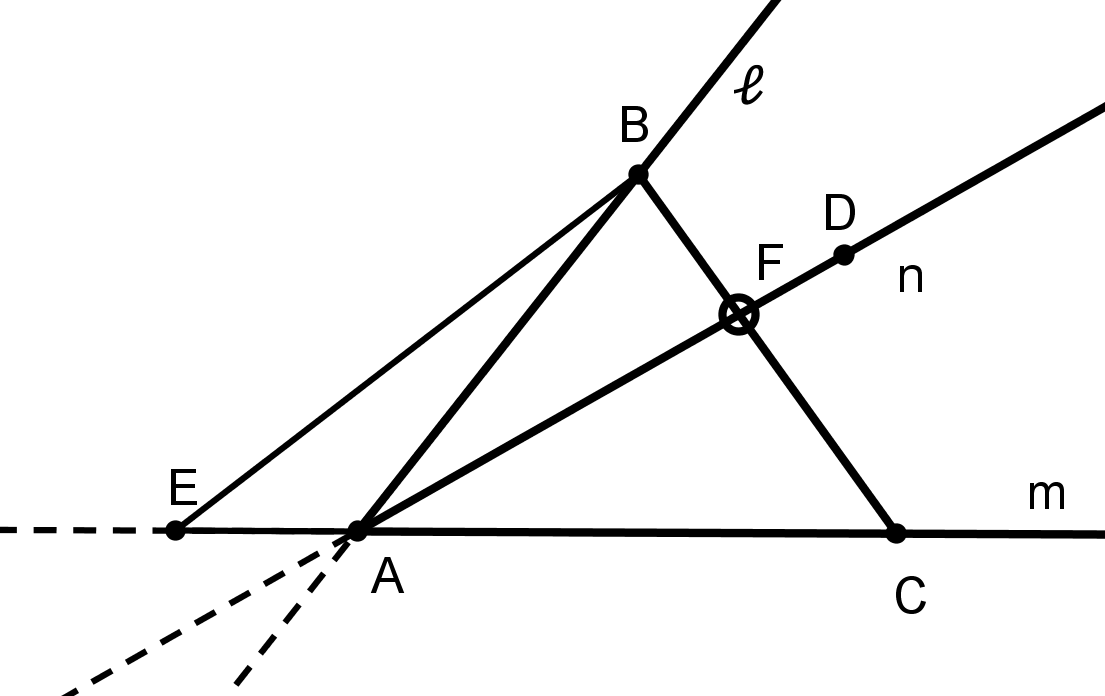
\includegraphics[width=8cm]{BILDER/1-1-09-Satz.png}}

    Die Strecke $\str{BE}$ liegt ganz auf einer Seite von $l$ und schneidet $l$ nur in $B$. Da $E$
    und $C$ auf verschiedenen Seiten von $l$ liegen, liegen alle Punkte von $\str{BE}$ auf der
    anderen Seite von $l$ wie $C$.
    \renewcommand{\labelenumi}{\arabic{enumi}.} % ändert die Nummerierung von (1) auf 1.
    \begin{enumerate}
        \item Der Strahl $\pf{AD}$ liegt im Innern des Winkels und damit ganz auf derselben Seite
            von $l$ wie $C$ (und auf derselben Seite von $m$ wie $B$) $\Rightarrow\;
            \pf{AD} \cap \str{EB} = \emptyset$.

        \item Entsprechend liegt der zu $\pf{AD}$ entgegengesetzte Strahl $\pf{AD}^* := \{X \, | \,
            \Zw(DAX)\}$ auf der anderen Seite von $m$ wie $\str{EB}$.
    \end{enumerate}
    Aus $1.$ und $2.$ folgt: $n \cap \str{EB} = \emptyset$ und daher $n \cap \str{BC} \neq
    \emptyset$, etwa $= \{F\}$.

    $F$ liegt auf $\pf{AD}$, denn $B$ und $F$ sowie $B$ und $D$ liegen auf derselben Seite von $m$,
    also auch $D$ und~$F$.
\end{proof}

\subsection{Kartesische Modelle mit Ordnung}

Ein Modell einer Ebene, die die Inzidenzaxiome erfüllt, ist die {\em kartesische Ebene} $\E_{_\K} =
\K^2$ über einem Körper $\K$.  Geraden werden, wie aus der Linearen Algebra bekannt, als Lösungen
linearer Gleichungen $a x + b y = c$ mit $a, b, c \in \R$ ($a, b$ nicht beide $0$) definiert.

Für endliche Körper erhalten wir endliche affine Geometrien, die aber nicht den Anordnungsaxiomen
genügen. Man betrachte beispielsweise "`Modell ~\ref{Modell2}"' auf Seite ~\pageref{Modell2}, dass
der kartesischen Ebene über dem Körper $\K = \{0, 1\}$ mit zwei Elementen entspricht: $\E_{\K} = \{A
= (0,0),\, B = (0,1),\, C = (1,0),\, D = (1,1)\}$.

\centerline{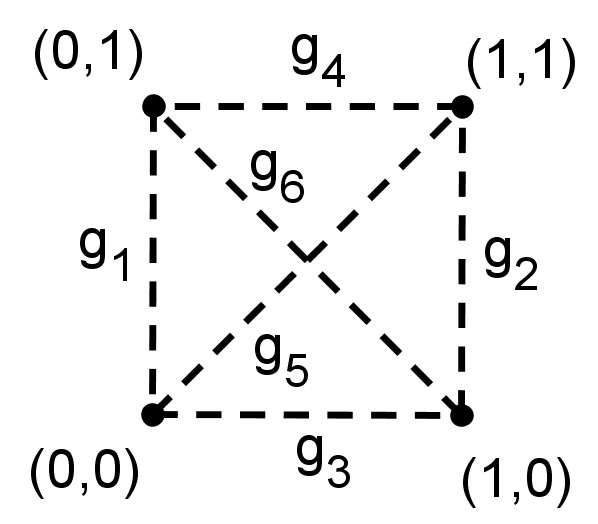
\includegraphics[width=5cm]{BILDER/1-1-10-Modell2.png}}

Es gibt allerdings eine Reihe von kartesischen Ebenen, die die Axiome der Anordnung ebenfalls
erfüllen.

\begin{defi}
    Ein Körper $K$ heißt {\em geordnet}, wenn er eine Teilmenge $K_+\subset K$ (von {\em positiven
    Elementen}) besitzt, so dass gilt:
    \renewcommand{\labelenumi}{(\roman{enumi})} % ändert die Nummerierung von (1) auf (i)
    \begin{enumerate}
        \item $\forall\, a,\, b \in K_+$ ist $a + b \in K_+$ und $a \cdot b \in K_+$;

        \item $\forall\, a \in K$ gilt genau eine der Beziehungen $a \in K_+$, $a = 0$ oder $-a \in
        K_+$.
    \end{enumerate}
\end{defi}

$\Q$ und $\R$ sind geordnet, $\C$ ist nicht geordnet.

Wenn $\K$ geordnet ist, können wir eine Ordnungsrelaton "`$<$"' definieren.
% Die Umkehrung gilt übrigens auch!! (Übung?!?)

\begin{defi}
    Sei $K$ geordnet und $a,\, b \in K$. Dann definieren wir:
    \begin{enumerate}
        \item $a > b\;: \Longleftrightarrow\; a - b \in K_+$;

        \item $a < b\;: \Longleftrightarrow\; b - a\in K_+$.
    \end{enumerate}
\end{defi}

Dies definiert eine {\em totale Ordnung} in $K$. Das heißt $\forall\, a,\, b \in K$ gilt genau eine
der Beziehungen: $a > b,\; a = b,\; a < b$.

\begin{thm}
    Sei $\K$ ein Körper und $\E_{\K}$ die entsprechende kartesische Ebene. Dann gilt:
    \begin{center}
        $\E_{\K}$ genügt den Axiomen der Anordnung $\Longleftrightarrow \K$ ist geordnet.
    \end{center}
\end{thm}

\begin{proof}
    \begin{itemize}
        \item["`$\Longrightarrow$"'] Wir betrachten die $x$-Achse $g$. Nach
            Theorem~\ref{thm:satz.s1b} wird $g$ durch $O = (0,0) \in g$ in 2 Seiten geteilt; sei

            \begin{align*}
                K_+ & := \{a \in \K:\; a \neq 0,\; (a,0) \mbox{ und } (1,0) \mbox{ liegen auf
                derselben Seite von } O\}\\
                -K_+ & := \{a \in \K:\; a \neq 0,\; (a,0) \mbox{ und } (1,0) \mbox{ liegen auf
                verschiedenen Seiten von } O\}
            \end{align*}

            Dann ist $\K = K_+ \cup \{0\} \cup -K_+$ eine disjunkte Vereinigung. Bleibt zu zeigen,
            dass mit $a, b\in K_+$ auch $a + b$ und $a \cdot b$ in $K_+$ liegen.

            \begin{description}
                \item[Addition] Die Addition $a + b$ in $\K$ entspricht dem nacheinander "`anlegen"'
                von Strecken der Längen $a$ und $b$ auf der $x$-Achse $g$ %der Addition von Strecken

                % XXX: HIER MUSS DEFINITIV NOCHMAL ÜBERDACHT WERDEN!!!!!
                % WAS SOLL UNS DAS SAGEN??? "entspricht Addition von Strecken?!?!
                % HIER BITTE EIN SAUBERES ARGUMENT!!!
                % Dieses Argument ist aus dem Buch von Hartshorne kopiert, aber nur weil die
                % "segment arithmetic" dort schon vorher behandelt wurde!!!
                % siehe Hartshorne, Proposition 15.3

                $\Rightarrow\; a + b \in K_+$

                \centerline{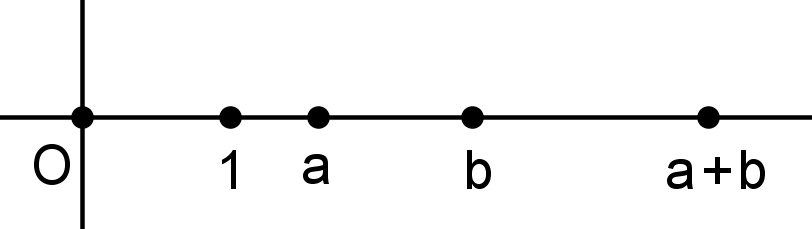
\includegraphics[width=6cm]{BILDER/1-1-16a-Satz.png}}

                \item[Multiplikation] Parallele durch $B = (0,b)$ zur Geraden durch die beiden
                    Punkte $E = (0,1),\; A = (a,0)$ schneidet $x$-Achse $g$ in $X = (a \cdot b, 0)$

                    % Beh.:  $a\cdot b\in K_+$

                    \centerline{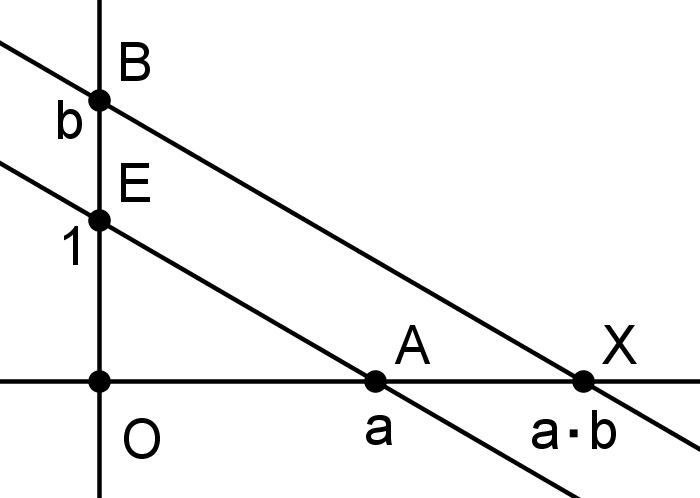
\includegraphics[width=6cm]{BILDER/1-1-16b-Satz.png}}

                    \renewcommand{\labelenumi}{\roman{enumi})} % Nummerierung: (1) -> 1)
                    \begin{enumerate}
                        \item Sei $\Zw(OEB)$ und $g(B,X)$ parallel zu $g(A,E)$. Dann liegen ganz
                            $g(B,X)$ und $O$ auf verschiedenen Seiten von $g(A,E)$, also auch
                            $\Zw(OAX)$.

                        \item Ist $\Zw(OBE)$ ergibt sich entsprechend $\Zw(OXA)$. In beiden Fällen
                            liegen daher $X$ und $A$ auf derselben Seite von $O$, also $a \cdot b
                            \in K_+$ und $K$ ist geordnet.
                    \end{enumerate}
            \end{description}

        \item["`$\Longleftarrow$"'] Sei $K$ geordnet und $A = (a_1,a_2),\; B = (b_1,b_2),\; C =
            (c_1,c_2)$ paarweise verschiedene Punkte einer Geraden $g:\; a x + b y + c = 0$.\\
            \textbf{Zwischenrelation:}

            \renewcommand{\labelenumi}{\arabic{enumi})} % ändert die Nummerierung von (1) auf 1)
            \begin{enumerate}
                \item Sei $b \neq 0: \quad \Zw(ABC)\;: \Leftrightarrow\; a_1 > b_1 > c_1$ oder
                    $a_1 < b_1 < c_1$;

                \item sei $b = 0\; (\mbox{d.h. } a_1 = b_1 = c_1 = \frac{-c}{a}):$

                    $\Zw(ABC)\;: \Leftrightarrow\; a_2 > b_2 > c_2$ oder $a_2 < b_2 < c_2$.
            \end{enumerate}

            Man prüft nun die Gültigkeit von (A1) - (A4) nach. % Übung, Blatt 3
    \end{itemize}
\end{proof}

\subsection*{Poincarésches Kreisscheibenmodell}

Ein weiteres Modell, dass den Inzidenz- und Anordnungsaxiomen genügt, ist das Poincarésche
Kreisscheibenmodell. Hierbei wählen wir die Menge der Punkte in einer offenen Kreisscheibe des
$\R^2$. (Anstelle des $\R^2$ ließe sich auch der $\K^2$ für einen anderen geordneten Köprper
verwenden.) Der Einfachheit halber wählen wir einen Kreis mit Mittelpunkt im Ursprung:
$$
    \Gamma = \{ (x,y) \in \R^2 :  x^2 + y^2 = r \}
$$
Punkte in unserem {\em  Poincaréschen Kreisscheibenmodell} sind also aus
$$
    \E = \{ (x,y) \in \R^2 :  x^2 + y^2 < r \}.
$$
Geraden sind Teile von Kreisen oder Geraden $\gamma$ des $\R^2$, die $\Gamma$ {\em orthogonal
schneiden}, d.h. die Tangenten an $\Gamma$ und $\gamma$ in den beiden Schnittpunkten liegen
orthogonal zueinander. Diese Orthogonalitätsbedingung ist im Fall einer Geraden $\gamma$ genau dann
erfüllt, wenn der Ursprung $O = (0,0)$ auf der Geraden liegt.

\centerline{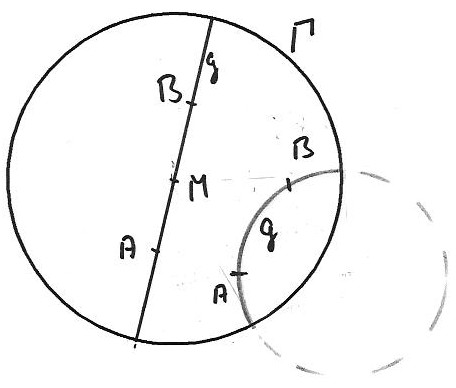
\includegraphics[width=6cm]{BILDER/4-2-04b-Geraden.jpg}}

\begin{thm} \label{thm:PoincareKreisscheibe}
    Das Poincarésche Kreisscheibenmodell genügt den Inzidenzaxiomen {\bf (I1) -- (I3)} und den
    Anordnungsaxiomen {\bf (A1) -- (A4)}.
\end{thm}

\subsection*{Inversion am Kreis}

Um zu zeigen, dass das Poincarésche Kreisscheibenmodell dem Inzidenz-Axiom {\bf (I1)} genügt,
benötigen wir zunächst ein paar Aussagen über sich orthogonal schneidende Kreise.

%% Folgendes kann man auch für beliebige Körper mit Ordnung und
%% ... machen  (Euklidische Körper!)

\begin{defi}
    $\Gamma \subset \R^2$ sei ein Kreis vom Radius $r$ und Mittelpunkt $M$. $A \in \R^2$ sei ein
    beliebiger Punkt, $A \neq M$. Sei $A' \in \pf{MA}$ derart, dass $|MA| \cdot |MA'| = r^2$
    %(solch ein Punkt $A'$ existiert stets!).
    Wir sagen, $A'$ entsteht aus $A$ durch eine \emph{Inversion} $\varphi_\Gamma :
    \R^2 \setminus\{M\} \to \R^2 \setminus \{M\}$ am Kreis $\Gamma$.
\end{defi}

\centerline{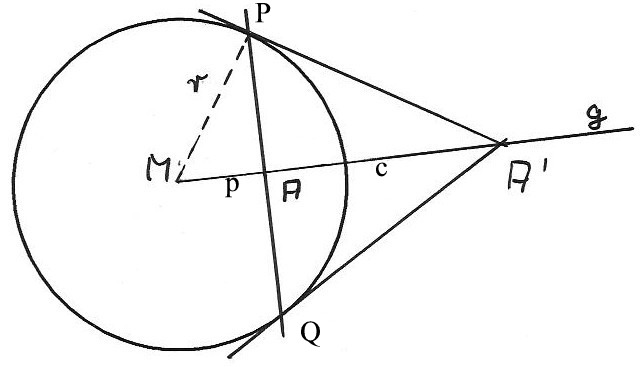
\includegraphics[width=8cm]{BILDER/4-2-01-Inversion.jpg}}

Die Punkte $A$ und $A'$ stehen in einer ganz besonderen Beziehung zueinander. Punkte außerhalb des
Kreises werden durch die Inversion am Kreis auf Punkte innerhalb des Kreises abgebildet und
umgekehrt. Liegt $A$ innerhalb des Kreises $\Gamma$, so bilden wir eine Gerade orthogonal zur
Geraden $g$ durch $M$ und $A$ durch $A$. Diese schneidet $\Gamma$ in zwei Punkten $P$ und $Q$. Die
Tangente an $\Gamma$ durch $P$ (orthogonal zu $g(M,P)$) trifft die Gerade $g$ in $A'$. Dies folgt
aus der Ähnlichkeit der Dreiecke $MPA'$ und $MAP$ und dem Verhältnis der Seitenlängen
$$
    \frac{|MA|}{r} = \frac{r}{|MA'|}.
$$
\begin{thm}\label{thm:satz.s4b}
    Inversionen $\varphi_\Gamma$ am Kreis $\Gamma$ haben folgende Eigenschaften:

    \renewcommand{\labelenumi}{\alph{enumi})} % ändert die Nummerierung von (1) auf a)
    \begin{enumerate}
        %\item[\emph{\textbf{a)}}] Kreise durch $M$ werden in Geraden $g$ mit $M\notin
        %    g$ abgebildet und umgekehrt.
        \item Ein Kreis $\gamma$, der $\Gamma$ orthogonal schneidet, wird auf sich abgebildet.

        \item Enthält ein Kreis $\gamma$ zwei einander zugeordnete Punkte $A$ und
            $A' = \varphi_\Gamma(A)$, dann schneiden sich $\gamma$ und $\Gamma$ orthogonal.

        %\item[\emph{\textbf{d)}}] Ist $\gamma$ ein Kreis und $M\notin\gamma$, dann ist
        %    $\gamma'=\varphi_\Gamma(\gamma)$ ebenfalls ein Kreis.
        %\item[\emph{\textbf{e)}}] Winkel bleiben invariant.
    \end{enumerate}
\end{thm}
%\ref{satz.s4b}

\begin{proof}
    \renewcommand{\labelenumi}{\alph{enumi})} % ändert die Nummerierung von (1) auf a)
    \begin{enumerate}
        \item Da sich $\Gamma$ und $\gamma$ orthogonal schneiden, stehen die Tangenten und Radien
            paarweise aufeinander senkrecht. Nach dem {\em Sehnen-Tangenten-Satz}
            %(Übung, Blatt 3!!)
            gilt
            $$
                |MA| \cdot |MA'| = |MP|^2 = r^2.
            $$
            \centerline{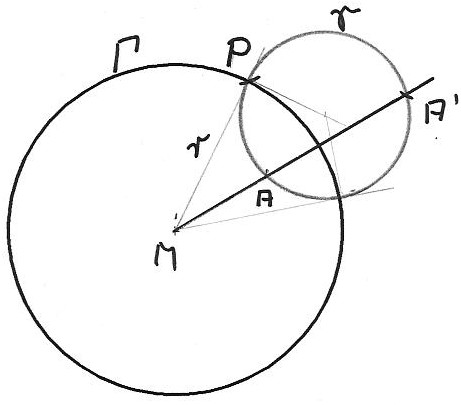
\includegraphics[width=6cm]{BILDER/4-2-02b-Inversion.jpg}}

        \item Gibt es umgekehrt $A,\, A' \in \gamma$ mit $|MA| \cdot |MA'| = r^2$, dann müssen sich
            $\Gamma$ und $\gamma$ schneiden. Sei $P$ ein Schnittpunkt von $\Gamma$ und $\gamma$.
            Dann ist $|MP| = r$, also $|MP|^2 = |MA| \cdot |MA'|$ und $|MP|$ ist Tangentenabschnitt
            für $\gamma$, auf dem der Radius von $\gamma$ orthogonal steht.
    \end{enumerate}
\end{proof}

Das Theorem zeigt insbesondere, dass das gesamte {\em Kreisbüschel} (Menge von Kreisen) durch zwei
Punkte $A$ und $\varphi_\Gamma(A)$ den Kreis $\Gamma$ orthogonal schneidet. Liegt $A$ im Inneren
der Kreisscheibe, so entsprechen die Schnitte des Kreisbüschels mit dem Inneren der Kreisscheibe,
allen Geraden durch $A$ im Poincaréschen Kreisscheibenmodel.

\centerline{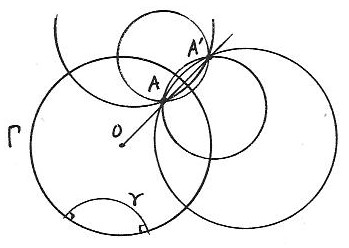
\includegraphics[width=6cm]{BILDER/4-2-06-Parallel.jpg}}

Betrachtet man eine Gerade $g$ (bzw. einen orthogonal schneidenden Kreis $\gamma$) außerhalb von
$A$, so sieht man auch, dass das Parallelenaxiom in der Poincaréschen Kreisscheibe nicht gilt.

\subsection*{Inzidenz und Anordnung im Kreisscheibenmodell}

Die Axiome der Inzidenz und Anordnung gelten allerdings in der Poincaréschen Kreisscheibe. Dazu
erklären wir die Beziehung "`Zwischen"' wie folgt: seien $A,\, B,\, C \in \E$ kollinear. Liegen
$A,\, B,\, C$ auf einem Durchmesser, also einer Geraden des $\R^2$, dann sei $Zw(ABC)$ wie im $\R^2$
erklärt. Liegen $A,\, B,\, C$ auf einem Kreis $\gamma$ mit Mittelpunkt $M'$, dann ziehen wir von
$M'$ die Strahlen zu $A,\, B,\, C$, diese treffen die Verbindungsstrecke der beiden Schnittpunkte
von $\gamma$ und $\Gamma$ in $A',\, B',\, C'$. Wir definieren $Zw(ABC)\; \Leftrightarrow\;
Zw(A'B'C')$ im Sinne des $\R^2$.

\centerline{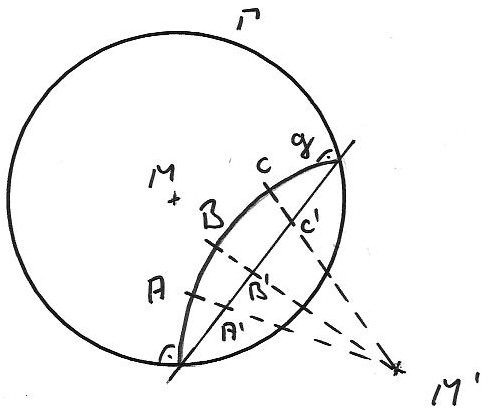
\includegraphics[width=6cm]{BILDER/4-2-07-Zwischen.jpg}}

\begin{proof}[Beweis von Theorem~\ref{thm:PoincareKreisscheibe}]
    {\bf (I2), (I3)} sind sicher erfüllt, genau so wie {\bf (A1) - (A3)}. %(Übung)??
    \begin{description}
        \item[(I1)] Seien $A,\, B \in \E$
            \begin{enumerate}
                \item $M,\, A,\, B$ kollinear $\Rightarrow\; \E$-Gerade ist der Durchmesser durch
                    $A$ und $B$.

                \item $M,\, A,\, B$ nicht kollinear, $A' = \varphi_\Gamma(A)\; \Rightarrow\;
                    \exists$ genau einen Kreis $\gamma$ durch $A,\, B,\, A'$, $\gamma$ ist
                    orthogonal zu $\Gamma$ nach Theorem~\ref{thm:satz.s4b}, b); ebenfalls $B' \in
                    \gamma$ nach Theorem~\ref{thm:satz.s4b} (a).
            \end{enumerate}
    \end{description}
\end{proof}

\begin{description}
    \item[(A4) -- Axiom von Pasch] Gegeben sei das Dreieck $ABC\subset\E$. Je 2 Geraden (Kreise)
        schneiden sich innerhalb $\Gamma$ in genau 1 Punkt $X$ (der 2. Schnittpunkt $X' =
        \varphi_\Gamma(X)$ liegt außerhalb von $\Gamma$ (Übungsaufgabe).
\end{description}

$\Rightarrow$ Inneres des Dreiecks $ABC$ ist wohldefiniert (2 Punkte auf derselben Seite der
$\E$-Geraden $\Longleftrightarrow$ beide Punkte innerhalb oder außerhalb des Kreises)

\centerline{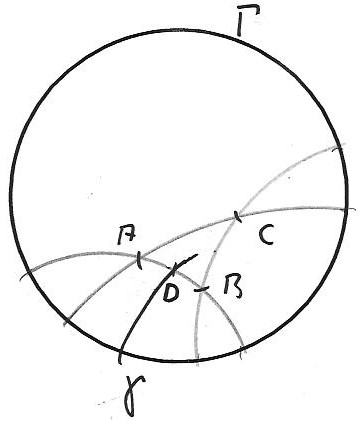
\includegraphics[width=5cm]{BILDER/4-2-08-Pasch.jpg}}

Ist $g$ eine $\E$-Gerade mit Kreis $\gamma$, die durch keinen der Eckpunkte $A,\, B,\, C$ geht und
etwa $\str{AB}$ in $D$ schneidet, dann liegen $A$ und $B$ auf verschiedenen Seiten von $g$, etwa $B$
innerhalb $\gamma$. Angenommen, $B,\, C$ auf derselben Seite von $\gamma$, etwa beide innerhalb
$\gamma\; \Rightarrow$ der Kreis durch $A,\, C$ enthält $A$ außerhalb und $C$ innerhalb von
$\gamma\; \Rightarrow\; \exists$ Schnittpunkt auf $AC$.

\section*{Vorlesung am 03.05.2011}
% Vertretung durch Thomas

\subsection*{Axiome der Kongruenz, Strecken}

Wir führen eine Relation zwischen Strecken (und später auch zwischen Winkeln) ein und nennen diese
"`Kongruenz"', in Zeichen $\str{AB} \cong \str{CD}$, wenn folgende Axiome erfüllt sind: 
%(Kongruenz ist in einem erweiterten Sinn eine "`{}Gleichheit"'{}):

\begin{enumerate}
    \item[{\bf (C1)}] (Existenz) Sei $\str{AB} \subset \E\; (A \neq B)$ und $C$ der Ursprung eines
        Strahls $r$. Dann gibt es genau einen Punkt $D \in r,\; D \neq C,$ mit $\str{AB} \cong
        \str{CD}$.

    %\includegraphics[width=3.5cm]{1-2-01-C1}

    \item[{\bf (C2)}] Wenn 2 Strecken einer dritten kongruent sind, dann sind sie zueinander kongruent:
        $$
            \str{AB} \cong \str{CD} \mbox{ und } \str{AB} \cong \str{EF}\; \Rightarrow\; \str{CD} \cong \str{EF}.
        $$
        Jede Strecke ist zu sich selbst kongruent.

    \item[{\bf (C3)}] (Addition) Wenn $A,\,B,\,C\in \E$ und $Zw(ABC)$\\
        sowie $D,\, E,\, F \in \E$ mit $Zw(DEF)$ und\\
        $\str{AB} \cong \str{DE}$, $\str{BC} \cong \str{EF}$, dann ist auch $\str{AC} \cong
        \str{DF}$.

    %\includegraphics[width=4cm]{1-2-01-C3}
\end{enumerate}

\begin{thm}\label{thm:satz.s1d}
    Die Kongruenz von Strecken ist eine Äquivalenzrelation.
\end{thm}
%\ref{satz.s1d}

\begin{proof}
    Übungsaufgabe.
\end{proof}

Die Definition der Kongruenz von Strecken erlaubt uns auch mit Strecken zu rechnen.

\begin{defi}[Addition von Strecken]\label{def:d1a}
    Seien $\str{AB}$ und $\str{CD}$ Strecken, $r = \pf{AB}$ ein Strahl. Ist $E$ der eindeutig
    bestimmte Punkt auf $r$, so dass $\str{BE} \cong \str{CD}$ nach \textbf{(C1)}, dann heißt
    $\str{AE}$ {\em die Summe von $\str{AB}$ und $\str{CD}$}:
    $$
        \str{AB} + \str{CD} := \str{AE}.
    $$
\end{defi}

\centerline{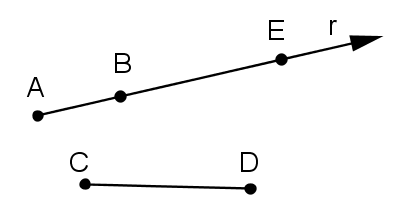
\includegraphics[width=5cm]{BILDER/1-2-02-Add.png}}

Die Addition ist eine wohldefinierte Operation auf den Äquivalenzklassen kongruenter Strecken, wie
die folgende Aussage belegt.

%% BEMERKUNG: Man kann auch zeigen, dass die Addition assoziativ und
%% als Operation auf den Äquivalenzklassen kommutativ ist.
%% Siehe Hartshorne, Excercise 8.1

\begin{thm}\label{thm:satz.s1e}
    Sei $\str{AB} \cong \str{A'B'}$ und $\str{CD} \cong \str{C'D'}\; \Longrightarrow\; \str{AB} +
    \str{CD} \cong \str{A'B'} + \str{C'D'}$

    Das heißt die Addition von Strecken ist unabhängig von den ausgewählten Repräsentanten.
\end{thm}
%\ref{satz.s1e}

\begin{proof}
    Sei $E$ wie in Definition~\ref{def:d1a}: $\str{AE} = \str{AB}+\str{CD}$ und entsprechend $E':$
    $$
        \str{A'E'} = \str{A'B'} + \str{C'D'}
    $$
    Daraus folgt $\str{BE} \cong \str{CD} \cong \str{C'D'} \cong \str{B'E'} \Longrightarrow\;
    \str{BE} \cong \str{B'E'}$ nach (\ref{thm:satz.s1d}) $\Longrightarrow$ (C3)
    $\str{AE}\cong\str{A'E'}$.

    \centerline{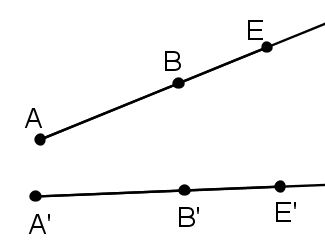
\includegraphics[width=5cm]{BILDER/1-2-03-Add.png}}
\end{proof}

\begin{thm}[Differenz von Strecken]\label{thm:satz.s1f}
    Seien $A,\, B,\, C$ kollinear mit $Zw(ABC)$ und $E,F$ seien zwei Punkte auf einem Strahl
    $\pf{DE}$ mit {\em Ausgangspunkt} $D$, so dass $\str{AB} \cong \str{DE}$ und $\str{AC} \cong
    \str{DF}$. Dann gilt $Zw(DEF)$ und $\str{BC} \cong \str{EF}$.  ($\str{BC}$ heißt
    \emph{Differenz} von $\str{AC}$ und $\str{AB}$.)
\end{thm}

\begin{proof}
    Sei $F'$ auf dem Strahl $\pf{DE}$ gewählt, so dass $Zw(DEF')$ und $\str{BC} \cong \str{EF'}$
    nach (C1) $\stackrel{(C3)}{\Longrightarrow}$ $\str{AC} \cong \str{DF'}$. Die Punkte $F$ und
    $F'$ liegen beide auf $\pf{DE}$. Ausserdem gilt $\str{AC} \cong \str{DF}$, so dass aus (C2) und
    der Eindeutigkeit in (C1), auch $F=F'$ folgt. Also auch $Zw(DEF)$.

    \centerline{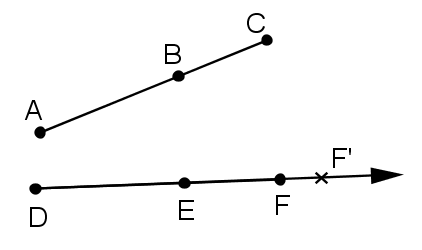
\includegraphics[width=5cm]{BILDER/1-2-04-Diff.png}}
\end{proof}

Es ist auch möglich Strecken miteinander zu vergleichen:

\begin{defi}
    Seien $\str{AB}$ und $\str{CD}$ Strecken in $\E$. Dann sei $\str{AB} < \str{CD}\;:
    \Leftrightarrow\; \exists\, E \in \str{CD},\; Zw(CED)$ und $\str{AB} \cong \str{CE}$.
\end{defi}

\centerline{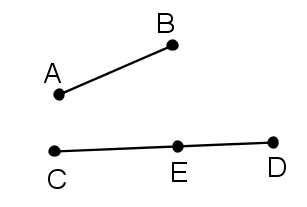
\includegraphics[width=5cm]{BILDER/1-2-05-Ord.png}}

\begin{thm}\label{thm:satz.s1g}\ % Das erzwungene Leerzeichen sorgt für den Umbruch.
    \renewcommand{\labelenumi}{\alph{enumi})} % ändert die Nummerierung von (1) auf a)
    \renewcommand{\labelenumii}{\alph{enumi}\textsubscript{\arabic{enumii}})}
        % Nummerierung 2. Ebene
    \begin{enumerate}
        \item\label{thm:satz.slg.item1} Ist $\str{AB} \cong \str{A'B'}$ und $\str{CD} \cong
            \str{C'D'}\; \Longrightarrow\; \{\str{AB} < \str{CD} \Leftrightarrow \str{A'B'} <
            \str{C'D'}\}$

        \item "`$ < $"' ist eine Ordnungsrelation in der Menge aller Strecken, d.h.
            \begin{enumerate}
                \item\label{thm:satz.slg.item2-1} $\str{AB} < \str{CD}$ und $\str{CD} < \str{EF}\;
                    \Longrightarrow \; \str{AB} < \str{EF}$

                \item\label{thm:satz.slg.item2-2} $\forall$ Strecken $\str{AB},\, \str{CD} \subset
                    \E$ gilt genau eine der Relationen

                    $\str{AB} < \str{CD},\; \str{AB} = \str{CD}$ oder $\str{AB}>\str{CD}$.
            \end{enumerate}
    \end{enumerate}
\end{thm}

\begin{proof}
    \begin{enumerate}
        \item[zu ~\ref{thm:satz.slg.item1}.]\ % erzwungenes Leerzeichen => Umbruch
            \begin{itemize}
                \item["`$\Longrightarrow$"'] Sei $\str{AB} < \str{CD} \Longrightarrow\; \exists\, E
                    \in \str{CD},\; Zw(CED)$ und $\str{AB} \cong \str{CE}\;
                    \stackrel{(C1)}{\Longrightarrow}\; \exists\, E' \in r':\; \str{CE} \cong
                    \str{C'E'}$ und $D',\, E'$ auf derselben Seite von $C'$.  Wegen $\str{CD} \cong
                    \str{C'D'}$ und Theorem~\ref{thm:satz.s1f} folgt $Zw(C'E'D')$ und $\str{A'B'}
                    \cong \str{CE} \cong \str{C'E'}$, also $\str{A'B'} < \str{C'D'}$.

                \item["`$\Longleftarrow$"'] genauso.

                \centerline{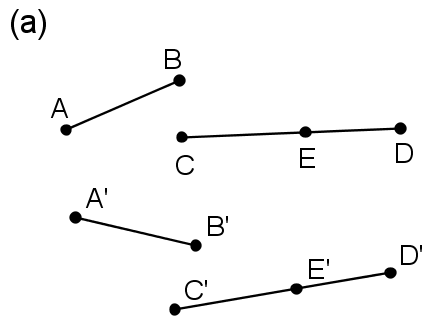
\includegraphics[width=5cm]{BILDER/1-2-06a-Ord.png}}
            \end{itemize}

            % \textbf{b)} Dem Beweis von b) stellen wir folgende Aussage voran:

            % \begin{lemma}\label{lemma.l1d}
            % Sind $A,B,C\in g$ kollinear und $Zw(ABC)$, dann liegen $A,\,B$ auf
            % derselben Seite von $C$ und $B,\,C$ auf derselben Seite von $A$
            % \emph{(sonst $Zw(ACB)$ bzw. $Zw(BAC)$)}. Gilt dann auch noch
            % $Zw(ACD)$, also $A$ und $D$ auf verschiedenen Seiten von $C$, dann
            % liegen $A$ und $D$ auch auf verschiedenen Seiten von $B$ und $B$
            % und $D$ auf verschiedenen Seiten von $C$, also $Zw(ABD)$ und
            % $Zw(BCD)$.
            % \end{lemma}
            % %\ref{lemma.l1d}
            % Wir haben das Bild: \qquad\qquad
            % \includegraphics[width=6cm]{1-2-07-Ord}

            % \textbf{Beweis zu \ref{lemma.l1d}} Mit den Bezeichnungen aus
            % Abschnitt 1.1 gilt:
            % \[Zw(ABC)\wedge Zw(ACD)\;\Longrightarrow\;A\stackrel{C}{\sim}
            % B\;\mbox{und}\;A\stackrel{C}{\nsim}D\;\Longrightarrow\;
            % B\stackrel{C}{\nsim}D\;\Longrightarrow\; Zw(BCD)\] und
            % \[Zw(BCD)\wedge Zw(ABC)\;\Longrightarrow\;C\stackrel{B}{\sim}
            % D\;\mbox{und}\;A\stackrel{B}{\nsim}C\;\Longrightarrow\;
            % A\stackrel{B}{\nsim}D\;\Longrightarrow\; Zw(ABD),\] qed.

        \item[zu ~\ref{thm:satz.slg.item2-1}.] Sei $\str{AB} \cong \str{CX}$ mit $Zw(CXD)$ sowie
            $\str{CD} \cong \str{EY}$ mit $Zw(EYF)$. Nach Theorem~\ref{thm:satz.s1f} gibt es ein $Z
            \in \str{EY}$ mit $\str{CX} \cong \str{EZ}$. Aus $Zw(EYF)$ und $Zw(EZY)$ folgt
            % aus Lemma \ref{lemma.l1d} 
            $Zw(EZF)$ (Übung). % ACHTUNG: Diese Aussage ist nicht trivial!
            Also $\str{AB} < \str{EF}$.

            \centerline{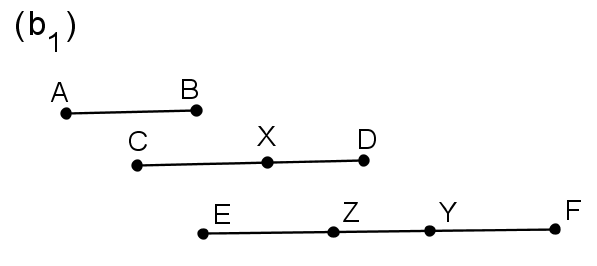
\includegraphics[width=5cm]{BILDER/1-2-06b1-Ord.png}}

        \item[zu ~\ref{thm:satz.slg.item2-2}.] Sei $r = \overrightarrow{CD}$ und $E \in r$ derart,
            dass $\str{AB} \cong \str{CE}\; \Longrightarrow\; Zw(CED)\; (\str{AB} < \str{CD})$ oder
            $E = D\; (\str{AB} \cong \str{CD})$ oder $Zw(CDE)\; (\str{AB} > \str{CD})$.

            \centerline{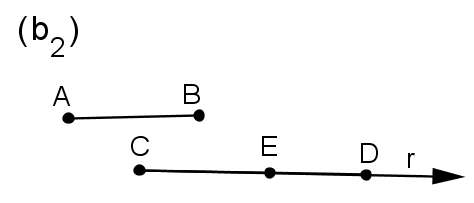
\includegraphics[width=5cm]{BILDER/1-2-06b2-Ord.png}}
    \end{enumerate}
\end{proof}

\subsection*{Kongruenz von Strecken für geordnete Körper}

Die Kongruenz von Strecken in der kartesischen Ebene $\K^2$ kann wie gewohnt über die {\em
Distanzfunktion} erklärt werden. Für zwei Punkte $A = (a_1,a_2)$ und $B = (b_1,b_2)$ ist die Distanz
erklärt durch
$$
    \dist(A,B) := \sqrt{(a_1-b_1)^2 + (a_2-b_2)^2} .
$$
Wenn die Wurzel und damit die Distanzfunktion im Körper $\K$ erklärt ist, erklären wir zwei Strecken
$AB$ und $CD$ {\em kongruent}, wenn $\dist(A,B) = \dist(C,D)$. Das ist natürlich genau dann der
Fall, wenn
$$
\dist^2(A,B) = (a_1 - b_1)^2 + (a_2 - b_2)^2 = (c_1 - d_1)^2 + (c_2 - d_2)^2 = \dist^2(C,D).
$$
Letztere Bedingung hat den Vorteil, dass sie auch in Körpern $\K$ definiert ist, in denen nicht alle
Wurzeln existieren.

%Wenn die Wurzel in $\K$ nicht erklärt ist, können wir Strecken $AB$ und $CD$ deshalb
%einfach kongruent erklären wenn die entsprechende Gleichheit für die
%Quadrate der Distanzfunktion gilt, d.h., wenn $\dist^2(A,B) =
%\dist^2(C,D)$.

Man könnte die Kongruenz auch über andere Distanzfunktionen erklären, etwa über
$$
    \dist_1(A,B) := |a_1 - b_1| + |a_2 - b_2|
$$
oder
$$
    \dist_{\infty}(A,B) := \sup \{ |a_1 - b_1|, |a_2 - b_2| \}.
$$
% ACHTUNG: Dabei bekäme man aber Geometrien heraus, die nicht isomorph
% zur oben erklärten sind!! (untereinander wären die beiden aber
% durchaus isomorph!)
% siehe Hartshorne, Übungen 8.7-8.9

Für einen geordneten Körper $\K$ gilt $\dist^2(A,B) > 0$ genau dann wenn $A, B\in \K^2$ verschieden
sind.

\begin{thm}
    In der kartesischen Ebene $\E_{\K} = \K^2$ über einem geordneten Körper $\K$ gelten die
    Kongruenzaxiome {\bf (C2)} und  {\bf (C3)}. Das Kongruenzaxiom {\bf (C1)} gilt genau dann, wenn
    es zu jedem Element $a \in \K$ auch die Wurzel von $1 + a^2$ in $\K$ gibt. ($\K$ heißt in diesem
    Fall {\em Pythagoreischer Körper}).
\end{thm}

Man beachte, dass wir im Kapitel über Euklids Elemente gesehen haben, dass die Konstruktionen mit
Zirkel und Lineal immer innerhalb eines {\em Pythagoreischen Körpers} stattfinden.

% d.h., wenn wir die Punkte mit denen wir beginnen aus $\K^2$ wählen, bleiben wir auch in $\K^2$...

\begin{proof}
    Das Kongruenzaxiom {\bf (C2)} ist eine einfache Folgerung aus der Definition von $\dist^2(A,B)$.
    Der Nachweis von {\bf (C3)} bleibt als Übungsaufgabe.

    %{\bf TO BE FILLED:  Parts of proof of Proposition 16.1 in Hartshorne!}

    Für die Äquivalenzaussage über {\bf (C1)} zeigen wir zunächst, dass die Aussage nicht für
    beliebige Körper gilt. Für $a\in \K$ betrachten wir dazu die Strecke $OA$ mit $O = (0,0)$ und $A
    = (a,1)$. Um zur Strecke $OA$ eine kongruente Strecke $OB$ auf der x-Achse "`abzutragen"',
    benötigen wir einen Punkt $B = (b,0)$ mit $\dist^2(O,A) = \dist^2(O,B)$, also mit
    $$
        1 + a^2 = b^2.
    $$
    Mit anderen Worten: Wir benötigen ein Element $b \in \K$, dass die Wurzel von $1 + a^2$ ist.

    Umgekehrt: Angenommen für jedes $c\in \K$ gibt es ein Element $\sqrt{1 + c^2} \in \K$. Dann
    können wir für jedes Paar $a, b \in \K$, mit $a \not = 0$, die Wurzel aus $a^2 + b^2$ in $\K$
    finden: Zunächst gilt
    $$
        a^2+b^2 = a^2 \left(1+ \left(\frac{b}{a}\right)^2 \right).
    $$
    Mit $c = b/a$ gilt dann
    $$
        \sqrt{a^2 + b^2} = |a| \cdot \sqrt{1 + c^2}.
    $$
    %% ACHTUNG: Ist der Betrag überhaupt in $K$ erklärt!!?? (Ja weil, $K$ geordnet).
    Man beachte: Der Betrag $|a|$ von $a$ erklärt ist weil $\K$ geordnet ist; und wir haben durch
    obiges Argument gezeigt, dass in {\em Pythagoreischen Körpern} $\K$ die Distanz $\dist(A,B)$ von
    Strecken in $\E_{\K}$ immer auch ein Element des Körpers ist.

    Sei $g$ eine Gerade in $\E_{\K}$ beschrieben durch $y = m x + b$, mit $m, b \in \K$. Für einen
    beliebigen Punkt $A = (a, m a + b)$ auf $g$ und ein $d \in \K$ wollen wir eine Strecke $AC$ der
    Länge $d$ auf $g$ abtragen. D.h., für $C = (c, m c + b)$ gilt
    $$
        \dist(AC) = \sqrt{(a - c)^2 + ( (m a + b) - (m c + b) )^2} = d,
    $$
    bzw.
    $$
        |a-c| \cdot \sqrt{1 + m^2} = d.
    $$
    Da $\sqrt{1 + m^2} \in \K$ nach Voraussetzung, lässt sich die letzte Gleichung in $\K$ nach $c$
    auflösen. Dabei erhalten wir zwei Lösungen für die beiden möglichen Richtungen, in denen die
    Strecke $AC$ abgetragen werden kann.
\end{proof}

\begin{bem}
    An dieser Stelle könnte man noch als zweites Beispiel die Kongruenz von Strecken in der
    Poincaréschen Kreisscheibe erklären. Dazu müsste man nur das Doppelverhältnis von vier Punkten
    in der Kartesischen Ebene definieren (siehe Hartshorne, S.339) und dann die ``$P$-Kongruenz'' am
    Kreis erklären (siehe Hartshorne, S.358). Ein Beweis, dass (C1) -- (C3) erfüllt sind, sollte an
    dieser Stelle nicht gegeben werden.
\end{bem}

\section*{Vorlesung am 05.05.2011}
% Vertretung durch Thomas

\subsection*{Kongruenz von Winkeln}

\begin{enumerate}
    \item[{\bf(C4)}] (Existenz) Gegeben sei der Winkel $\wi(BAC)$ und ein Strahl $\pf{DE}$. Dann
        existiert ein eindeutig bestimmter Strahl $\pf{DF}$ auf einer vorgegebenen Seite von
        $g(D,E)$, so dass $\wi(BAC) \cong \wi(EDF)$.

        \centerline{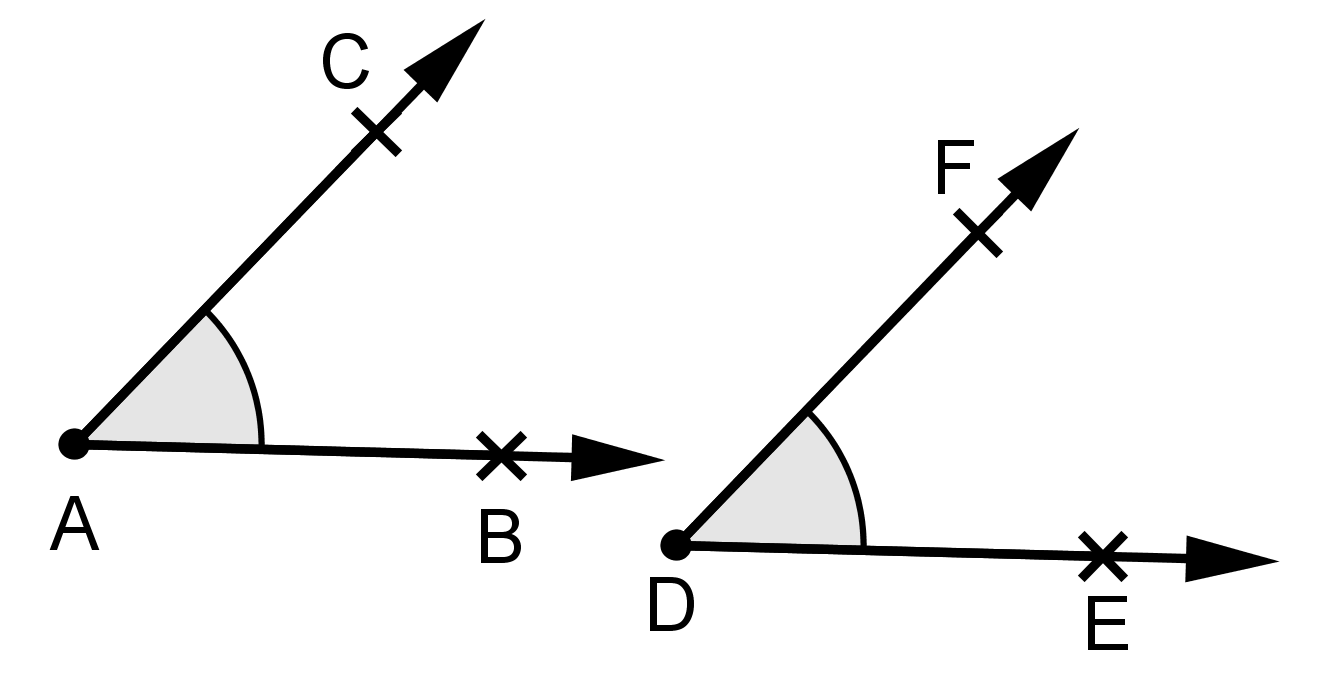
\includegraphics[width=5cm]{BILDER/1-2-08-C4.png}}

    \item[{\bf(C5)}] Für je 3 Winkel $\alpha,\, \beta,\, \gamma$ gilt: $\alpha \cong \beta$ und
        $\alpha \cong \gamma\; \Longrightarrow\; \beta \cong \gamma$\\

        %% KOMMENTAR NESSELMAN: (Woher?? Warum??)
        %    (Diese Aussage ist aus dem Rest beweisbar, so ist es aber bequemer!)\\
        %
        % FOLGENDE Reflexivität war im Nesselmann-Skript Teil von C4!?!?
        % Wir folgen hier Hartshorne...

        Jeder Winkel ist zu sich selbst kongruent: $\wi(BAC) \cong \wi(BAC)$.

    \item[{\bf(C6)}] Gilt für 2 Dreiecke $ABC$ und $DEF$: $\str{AB} \cong \str{DE},\; \str{AC} \cong
        \str{DF}$ und $\wi(BAC) \cong \wi(EDF)\; \Longrightarrow\; \wi(ABC) \cong \wi(DEF)$

        % (und damit durch Bezeichnungswechsel auch
        % $\wi(BCA)\cong\wi(EFD)\;\Longrightarrow$
        % die Dreiecke sind "`{}kongruent"'{})
        % Beweis siehe Hilbert \cite{Hil}, I.5)

    \centerline{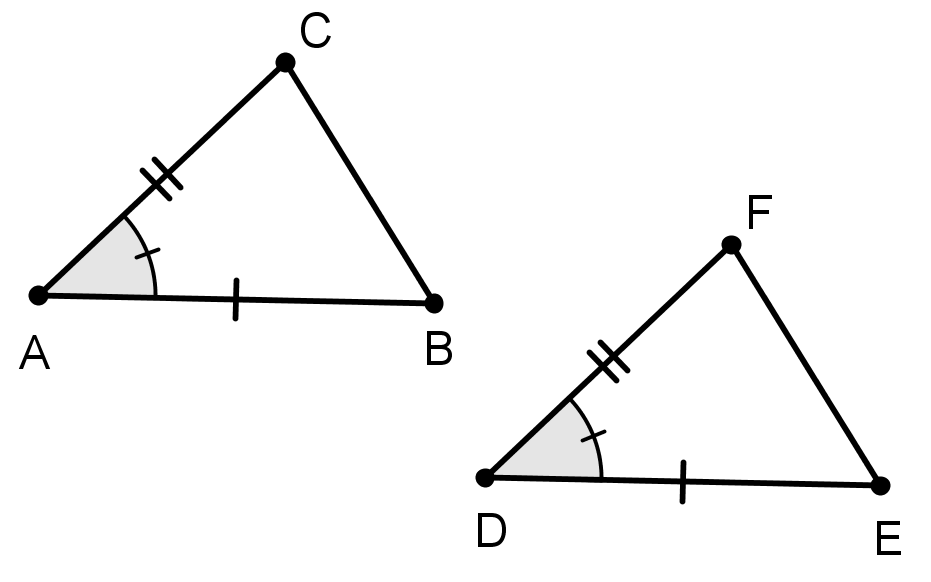
\includegraphics[width=5cm]{BILDER/1-2-08-C6.png}}
\end{enumerate}

\begin{bem}
    \renewcommand{\labelenumi}{\alph{enumi})} % ändert die Nummerierung von (1) auf a)
    \begin{enumerate}
        \item Nach den Kongruenzaxiomen wird weder der Strecke noch dem Winkel eine Richtung
            (Orientierung) zugeordnet.

        \item Axiom (C6) gewährleistet die Homogenität der Ebene, d.h. die Ebene verhält sich an
            jedem Punkt gleich.

        \item Die Kongruenzrelation der Winkel ist eine äquivalenzrelation (direkte Folge aus (C5)).
    \end{enumerate}
\end{bem}

\begin{defi}[Hilbert-Ebene]
    Eine Ebene, in der die Axiome {\bf (I1) -- (I3)}, {\bf (A1) -- (A4)} und {\bf (C1) --(C6)}
    gelten, heißt {\em Hilbert-Ebene}.
\end{defi}

\begin{bem}
    An dieser Stelle sollte man erklären, dass sich die Kongruenz von Winkeln in Kartesischen Ebenen
    $\E_{\K}$ über den Tangenz erklären lässt (siehe Hartshorne, S.141ff). Der Nachweis, dass (C6)
    gültig ist, ist dann etwas aufwendiger. Die Kongruenz von Winkeln in der Poincaréschen
    Kreisscheibe ist wie in der Kartesischen Ebene erklärt. An dieser Stelle sollte man es deshalb
    wohl dabei belassen zu erwähnen, dass es diese beiden Besipiele gibt (ohne es zu beweisen).
\end{bem}

%% Vgl. dazu Stillwell, Section 3.5!

\subsection*{Kongruenz von Dreiecken}

Ein wesentlicher Teil der aus der euklidischen Geometrie bekannten Dreiecksgeometrie lässt sich
bereits in einer Hilbert-Ebene beweisen.

% und ist damit Bestandteil der absoluten Geometrie.
% WAS SOLL DAS DENN HEISSEN?? Niemand weiß was "absolute Geometrie"
% ist an dieser Stelle...

% ACHTUNG: Die kurze Notation  $\wi{A}$, etc... wird ab hier immer
% wieder verwendet! Sollte vielleicht drauf hingewiesen werden...

\begin{defi}[Kongruenz von Dreiecken]
    Zwei Dreiecke $ABC$ und $DEF$ heißen {\em kongruent} $:\Longleftrightarrow$\\
    $\str{AB} \cong \str{DE},\; \str{AC} \cong \str{DF},\; \str{BC} \cong \str{EF}$ und $\wi{A}
    \cong \wi{D},\; \wi{B} \cong \wi{E},\; \wi{C} \cong \wi{F}$, d.h. Seiten und Winkel sind
    paarweise zueinander kongruent: $ABC \cong DEF$
\end{defi}

\centerline{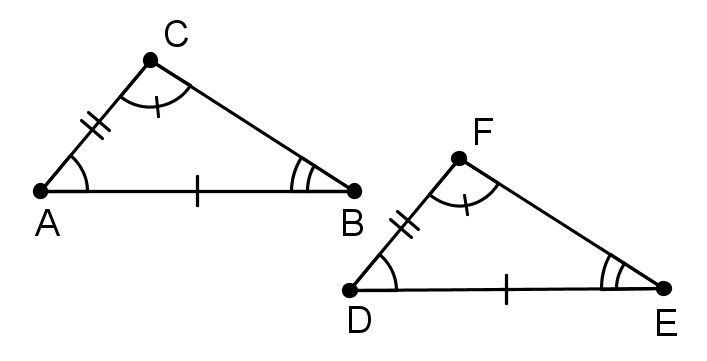
\includegraphics[width=5cm]{BILDER/1-2-09-Kongruenz.png}}

\begin{thm}[SWS-Kriterium]\label{thm:satz.s1h}
    Dreiecke, die den Bedingungen von {\bf (C6)} genügen, sind kongruent.
\end{thm}
%\ref{satz.s1h}

\begin{proof}
    Nach (C6) ist $\wi B \cong \wi E$ und $\wi C \cong \wi F$. Wir müssen noch $\str{BC} \cong
    \str{EF}$ zeigen.

    Sei $F'$ derart, dass $\str{BC} \cong \str{EF'}$ und etwa $F'\neq F$
    $\stackrel{(C6)}{\Longrightarrow} \wi(BAC) \cong \wi(EDF')$ und nach Voraussetzung $\wi(BAC)
    \cong \wi(EDF)$ im Widerspruch zu (C4) $\Longrightarrow\; F' = F$.
\end{proof}

\centerline{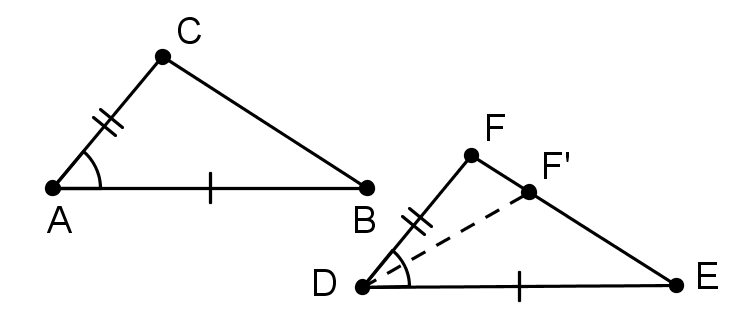
\includegraphics[width=5cm]{BILDER/1-2-10-SWS.png}}

Genauso erhält man:

\begin{thm}[WSW-Kriterium]\label{thm:satz.s1i}
    Gelten für 2 Dreiecke $ABC$ und $DEF$ die Kongruenzen $\str{AC} \cong \str{DF},\;\wi A \cong \wi
    D,\; \wi B \cong \wi E\; \Longrightarrow\; ABC \cong DEF$, d.h. die Dreiecke sind kongruent.
\end{thm}
%\ref{satz.s1i}

\begin{proof}
    Wie oben tragen wir $\str{BC}$ auf dem Strahl $\pf{EF}$ ab $\Longrightarrow\; \exists\, F':\;
    \str{BC} \cong \str{EF'}\; \stackrel{(C6)}{\Longrightarrow} \; ABC \cong DEF'$ und $\wi(EDF')
    \cong \wi(BAC) \cong \wi(EDF)$.

    Falls $F' \neq F\; \Longrightarrow\; \wi(EDF') < \wi(EDF)$ oder $\wi(EDF') > \wi(EDF)$ -
    Widerspruch.
\end{proof}

\centerline{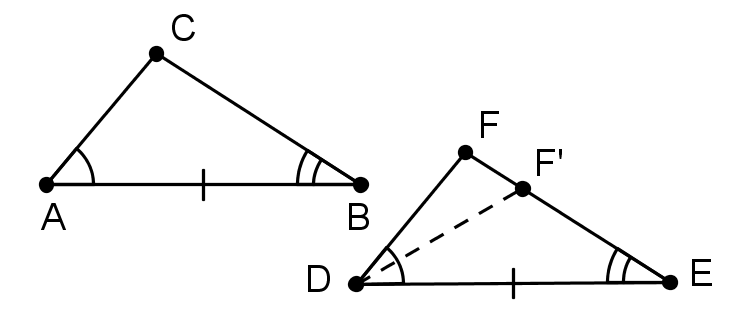
\includegraphics[width=5cm]{BILDER/1-2-11-WSW.png}}

\begin{thm}[SSS-Kriterium]\label{thm:satz.s1n}
    Wenn in zwei Dreiecken $ABC$ und $A'B'C'$ gilt $\str{AB} \cong \str{A'B'},\; \str{AC} \cong
    \str{A'C'}$ und $\str{BC} \cong \str{B'C'}$, dann ist $ABC \cong A'B'C'$.
\end{thm}
%\ref{satz.s1n}

Für den Beweis des SSS-Kriteriums benötigt man erheblich mehr Aufwand. Wir kommen darauf zurück\dots

\subsection*{Rechnen mit Winkeln}

Wie bei den Kongruenzaxiomen für Strecken, lassen sich auch für Winkel Summe, Differenz und eine
Ordnungsrelation erklären.

\begin{defi}\
    \renewcommand{\labelenumi}{\alph{enumi})} % ändert die Nummerierung von (1) auf a)
    \begin{description}
        \item[Summe von 2 Winkeln] Sei $\wi(BAC)$ ein Winkel und \pf{AD} ein Strahl im Innern, dann
            heißt $\wi(BAC)$ die Summe von $\wi(BAD)$ und $\wi(DAC)$.

            \centerline{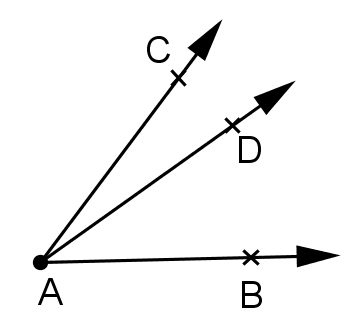
\includegraphics[width=5cm]{BILDER/1-2-12a-Winkel.png}}

        \item[Nebenwinkel] Sei $\wi(BAC)$ ein Winkel und $D \in g(A,C)$ auf der anderen Seite von
            $A$ wie $C$. Die Winkel $\wi(BAC)$ und $\wi(BAD)$ heißen \emph{Nebenwinkel}.

            %% ACHTUNG:
            % Hier sollte ein Bild zur Definition des Nebenwinkels hin, mit
            % C,A,D auf einer Geraden ; entsprechend sollte das Bild (die
            % Bezeichnungen) zur Definition des Rechten Winkels angepasst werden!

        \item[Scheitelwinkel] $\wi(BAC)$ und $\wi(DAE)$ heißen \emph{Scheitelwinkel}.

            \centerline{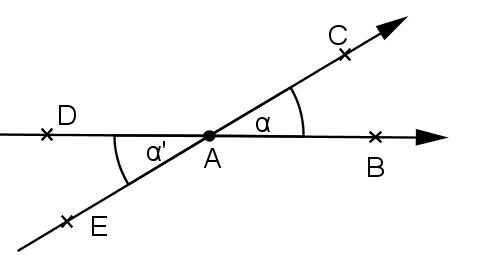
\includegraphics[width=5cm]{BILDER/1-2-12c-Winkel.png}}

        \item[rechter Winkel -- Rechter] $\alpha$ heißt ein \emph{rechter Winkel} oder
            \emph{Rechter} $:\Longleftrightarrow\; \alpha$ ist zu seinem Nebenwinkel kongruent
            ($\alpha\cong\beta$).

        \centerline{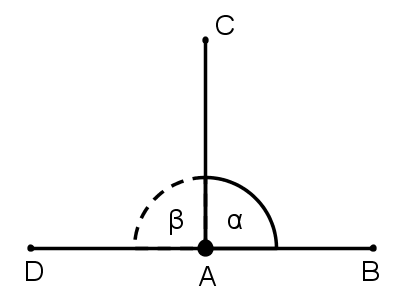
\includegraphics[width=5cm]{BILDER/1-2-12d-Rechter.png}}
    \end{description}
\end{defi}

\begin{thm}\label{thm:satz.s1k}
    Sind $\wi(BAC)$ und $\wi(BAD)$ sowie $\wi(B'A'C')$ und $\wi(B'A'D')$ paarweise Nebenwinkel und
    $\wi(BAC) \cong \wi(B'A'C')\; \Longrightarrow\; \wi(BAD) \cong \wi(B'A'D')$.
\end{thm}
%\ref{satz.s1k}

\begin{proof}
    Wir wählen $B',\, C',\, D'$ jeweils auf den entsprechenden Strahlen, so dass

    $\str{AB} \cong \str{A'B'}$, $\str{AC} \cong \str{A'C'}$, $\str{AD} \cong \str{A'D'}$ (nach
    (C1)).

    Das SWS-Kriterium~\ref{thm:satz.s1h} mehrfach anwenden ergibt:

    \renewcommand{\labelenumi}{\arabic{enumi}.} % ändert die Nummerierung von (1) auf 1.
    \begin{enumerate}
        \item $BAC\cong B'A'C'$

        \item $\str{DC}\cong\str{D'C'}$ nach (C3) $\stackrel{(SWS)}{\Longrightarrow}$

            $BCD \cong B'C'D'\; \Longrightarrow$

            $\wi(BDA) \cong \wi(B'D'A')$ und $\str{BD} \cong \str{B'D'}$ $\Rightarrow$

        \item $BDA \cong B'D'A'$

            $\Longrightarrow\; \wi(BAD) \cong \wi(B'A'D')$

    \end{enumerate}

    \centerline{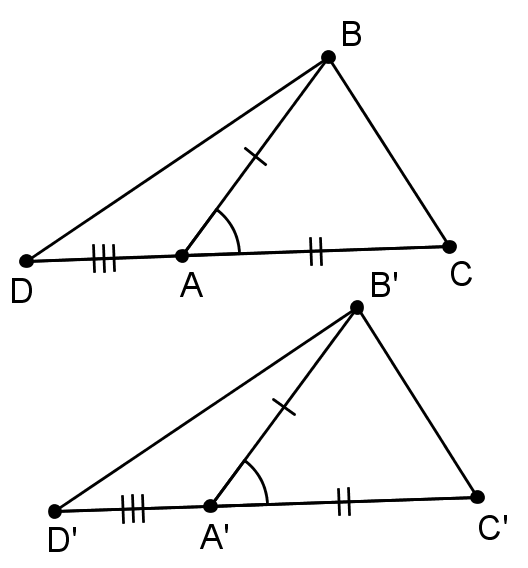
\includegraphics[width=5cm]{BILDER/1-2-13-Nebenwinkel.png}}
\end{proof}

% Folgendes mehr hervorheben?? Das ist ein Satz bei Hartshorne??
% Siehe seine Bemerkung ("Note") auf Seite 93, dass hier Euklid's
% I.13 ersetzt wird

Eine direkte Konsequenz des Theorems ist, dass Scheitelwinkel $\alpha$ und $\alpha'$ zueinander
kongruent sind. Sie sind nämlich beide Nebenwinkel eines Winkels $\beta$.

\begin{thm}\label{thm:satz.s1l}
    Mit den Bezeichnungen aus der Skizze gilt:

    %% Achtung: Hier sollte man vielleicht einen Text in die Aussage schreiben
    % (wie bei Hartshorne, S.93)

    \centerline{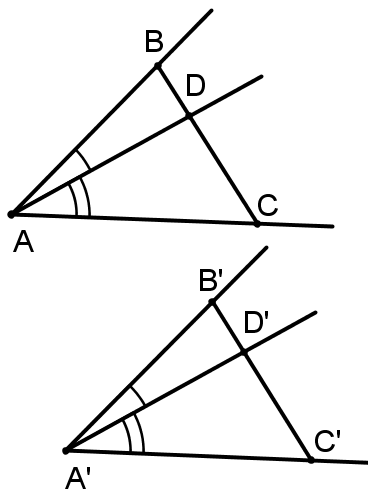
\includegraphics[width=5cm]{BILDER/1-2-15b-Winkel.png}}

    \renewcommand{\labelenumi}{\alph{enumi})} % ändert die Nummerierung von (1) auf a)
    \begin{enumerate}
        \item\label{thm:satz.s1l:item1} \emph{(Addition von Winkeln)} $\wi(BAD) \cong \wi(B'A'D')$
            und $\wi(DAC) \cong \wi(D'A'C')$\\ $\Rightarrow\;\wi(BAC) \cong \wi(B'A'C')$

        \item\label{thm:satz.s1l:item2} \emph{(Subtraktion von Winkeln)} $\wi(BAC) \cong
            \wi(B'A'C')$ und $\wi(DAC) \cong \wi(D'A'C')$\\
            $\Rightarrow\; \wi(BAD) \cong \wi(B'A'D')$
    \end{enumerate}
\end{thm}

$\wi(BAD)$ heißt die \emph{Differenz} der Winkel $\wi(BAC)$ und $\wi(DAC)$:
$$
    \wi(BAC) - \wi(DAC) := \wi(BAD).
$$
\begin{proof}
    \begin{description}
        \item[~\ref{thm:satz.s1l:item2}] Seien $B',\, C'$ so gewählt, dass $\str{AB} \cong
            \str{A'B'}$ und $\str{AC} \cong \str{A'C'} \stackrel{(SWS)}{\Longrightarrow} ABC \cong
            A'B'C'$ und daher $\wi(ABC) \cong \wi(A'B'C'),\; \wi(ACB) \cong \wi(A'C'B')$ und
            $\str{BC} \cong \str{B'C'}$ $\stackrel{(WSW)}{\Longrightarrow} ACD \cong  A'C'D'$ und
            somit $\str{CD} \cong \str{C'D'}$ und daher als Differenz kongruenter Strecken $\str{BD}
            \cong \str{B'D'}$
            % THOMAS (?) Sollte das folgende nicht \stackrel{(SWS)} sein???
            $\stackrel{(WSW)}{\Longrightarrow} BAD \cong B'A'D'$ und folglich $\wi(BAD) \cong
            \wi{B'A'D'}$.

        \item[~\ref{thm:satz.s1l:item1}] Als Nebenwinkel zu den kongruenten Winkeln $\alpha$ und
            $\alpha'$ ergibt sich wegen Theorem~\ref{thm:satz.s1k} die Kongruenz $\wi(DAE) \cong
            \wi(D'A'E')$ und daher nach ~\ref{thm:satz.s1l:item2}
            $$
                \beta = \wi(CAE) = \wi(DAE) - \wi(DAC) \cong \wi(D'A'E') - \wi(D'A'C') = \wi(C'A'E') =
                \beta'.
            $$
            Wiederum aus Theorem~\ref{thm:satz.s1k} folgt die Kongruenz $\wi(BAC) \cong \wi(B'A'C')$
            für die Nebenwinkel von $\beta$ und $\beta'$.

            \centerline{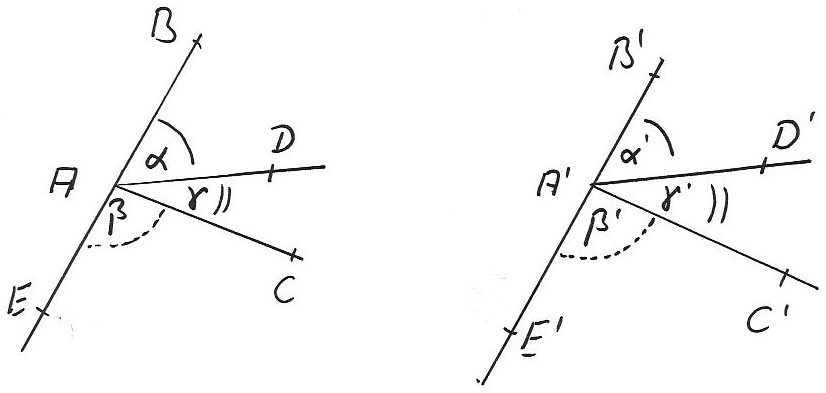
\includegraphics[width=7cm]{BILDER/1-2-15a-Winkel.jpg}}
    \end{description}
\end{proof}

\begin{defi}
    Gegeben seien zwei Winkel $\wi(BAC)$ und $\wi(EDF)$. Der Winkel $\wi(BAC)$ heißt kleiner als der
    Winkel $\wi(EDF)$, wenn es einen Strahl $\pf{DG}$ im Innern von $\wi(EDF)$ gibt, so dass
    $\wi(BAC) \cong \wi(GDF)$. $\wi(EDF)$ heißt größer als $\wi(BAC)$.
\end{defi}

\centerline{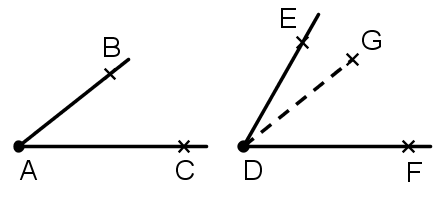
\includegraphics[width=5cm]{BILDER/1-2-16-Winkel.png}}

\begin{thm}\
    \renewcommand{\labelenumi}{\alph{enumi})} % ändert die Nummerierung von (1) auf a)
    \renewcommand{\labelenumii}{\alph{enumi}\textsubscript{\arabic{enumii}})}
        % ändert Nummerierung 2. Ebene
    \begin{enumerate}
        \item Ist $\alpha \cong \alpha'$ und $\beta \cong \beta'\;\Rightarrow$ $\{\alpha < \beta\;
            \Longleftrightarrow\; \alpha' < \beta'\}$.

        \item "`$ < $"' definiert eine Ordnung auf der Menge der Winkel, d.h.
        \begin{enumerate}
            \item $\alpha < \beta$ und $\beta < \gamma\; \Rightarrow\; \alpha < \gamma$.

            \item $\forall$ Winkel $\alpha$ und $\beta$ gilt genau eine der Beziehungen: $\alpha <
                \beta,\;\alpha \cong \beta,\;\alpha > \beta$.
        \end{enumerate}
    \end{enumerate}
\end{thm}

\begin{proof}
    Verläuft entsprechend wie der Beweis von Theorem~\ref{thm:satz.s1g} für Strecken. %(Übung?)
\end{proof}

% BEMERKUNG: Folgendes sind bei Euklid noch implizite Annahmen oder Axiome (CHECK!)

\begin{thm}\label{thm:satz.s1m}\
    \renewcommand{\labelenumi}{\alph{enumi})} % ändert die Nummerierung von (1) auf a)
    \begin{enumerate}
        \item Es gibt rechte Winkel.

        \item Je 2 rechte Winkel sind zueinander kongruent.
    \end{enumerate}
\end{thm}

\begin{proof}
    \renewcommand{\labelenumi}{\alph{enumi})} % ändert die Nummerierung von (1) auf a)
    \begin{enumerate}
        \item $C$ sei derart, dass $\str{OB} \cong \str{OC}$, $D$ sei der Schnittpunkt der Strecke
            $\str{BC}$ mit $\pf{OA}$

            \begin{enumerate}
                \item $D = O\in g(B,C)\; \Rightarrow\; \wi(BOA) \cong \wi(COA)$ und damit Rechter.

                \item $D \neq O \notin g(B,C)\; \Rightarrow\; BOD \cong COD\; \Rightarrow\; \wi(ODB)
                    \cong \wi(ODC)$ und damit Rechter.
            \end{enumerate}

            \centerline{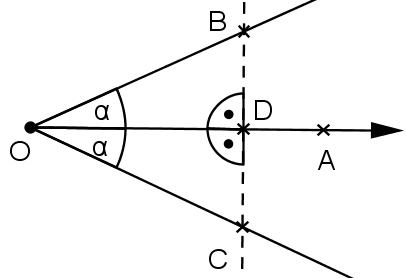
\includegraphics[width=5cm]{BILDER/1-2-18a-Winkel.png}}

        \item Angenommen, $\alpha \neq \alpha'$ seien verschiedene rechte Winkel, etwa $\alpha <
            \alpha'\; \Rightarrow$ tragen $\alpha$ am Strahl $\pf{A'B'}$ an und erhalten $\alpha
            \cong \wi(E'A'B')$ und $\pf{A'E'}$ im Innern von $\alpha'\; \Rightarrow\; C'$ im Innern
            von $\wi(E'A'D') \cong \beta\; \Rightarrow\; \beta' < \beta$.

            Jedoch: $\alpha' \cong \beta' < \beta \cong \alpha\; \Rightarrow\; \alpha' < \alpha$,
            Widerspruch.

            \centerline{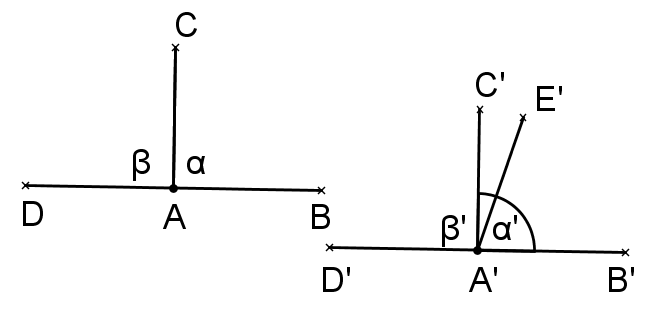
\includegraphics[width=5cm]{BILDER/1-2-18b-Winkel.png}}
    \end{enumerate}
\end{proof}

\section*{Vorlesung am 10.05.2011}

\subsection*{Beweis des SSS-Kriteriums}

Die Addition von Winkeln erlaubt auch einen Beweis des SSS-Kriteriums (Theorem~\ref{thm:satz.s1n}).
Zur Vorbereitung zunächst zwei Aussagen über gleichschenklige Dreiecke.

\begin{thm}\label{thm:lemma.l1b}
    Gilt in einem Dreieck $ABC$ die Kongruenz $\str{AC} \cong \str{BC}$, dann ist auch $\wi(CAB)
    \cong \wi(CBA)$, d.h. das Dreieck ist gleichschenklig. Umgekehrt folgt aus der Kongruenz der
    Winkel $\wi A \cong \wi B$ die Kongruenz der Seiten $\str{AC} \cong \str{BC}$.
\end{thm}
%\ref{lemma.l1b}

\begin{proof}
    Mit $B' = A,\;A' = B$ und $C' = C$ ist in beiden Fällen $ABC \cong A'B'C'$ - im 1. Fall wegen
    (SWS) und im 2. Fall wegen (WSW).
\end{proof}

\begin{thm}[Existenz gleichschenkliger Dreiecke]\label{thm:folg.f1a}
    Zu jeder Strecke $\str{AB}$ gibt es ein gleichschenkliges Dreieck mit $\str{AB}$ als Grundseite.
\end{thm}
%\ref{folg.f1a}

\begin{proof}
    Sei $\str{AB}$ gegeben und $C \notin g(A,B)$. Dann gibt es ein Dreieck $\triangle= ABC$. Wenn
    $\wi(CAB)\cong\wi(CBA)$, dann ist $\triangle$ gleichschenklig nach Theorem~\ref{thm:lemma.l1b}.
    Andernfalls sei etwa $\wi(CAB) < \wi(CBA)$.  Dann tragen wir gemäß (C4) den Winkel $\wi(CAB)$
    bei $B$ ab. Der zweite Schenkel $\pf{BE}$ schneidet nach \ref{thm:satz.s1c}. Die Strecke
    $\str{AC}$, etwa im Punkt $D$. Dann ist wieder nach Theorem~\ref{thm:lemma.l1b} $ABD$
    gleichschenklig.

    \centerline{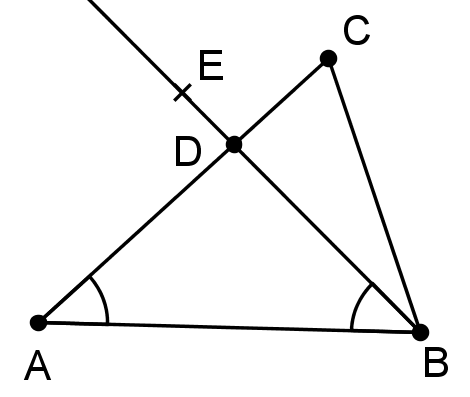
\includegraphics[width=5cm]{BILDER/1-2-20-Dreieck.png}}
\end{proof}

\begin{proof}[Beweis des SSS-Kriteriums, Theorem~\ref{thm:satz.s1n}]
    Es ist zu zeigen, dass sich die Kongruenz der Seiten auf die Winkel überträgt.

    \centerline{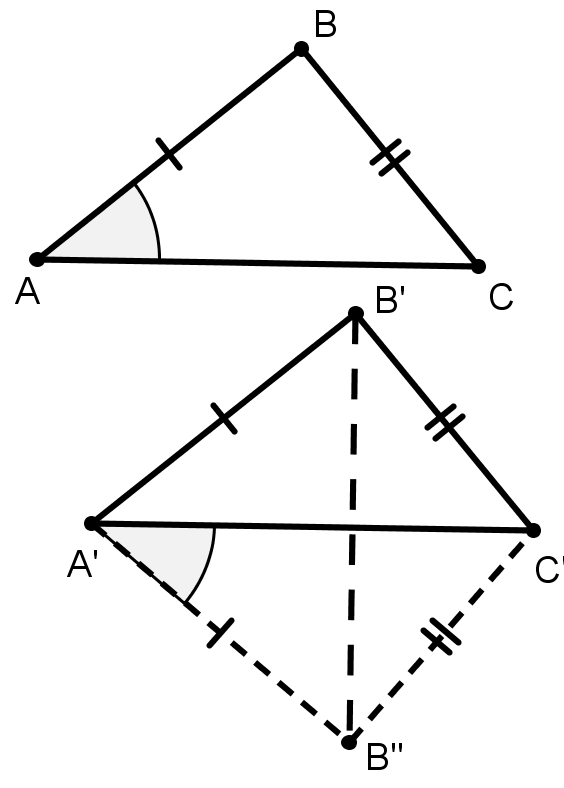
\includegraphics[width=5cm]{BILDER/1-2-21-SSS.png}}

    Sei $B''$ derart, dass $\wi(BAC) \cong \wi(B''A'C')$ und $\str{AB} \cong \str{A'B''}$

    $\stackrel{(SWS)}{\Longrightarrow}\; ABC \cong A'B''C'\; \Rightarrow\;\str{BC} \cong
    \str{B''C'}$

    $B'A'B''$ und $B'C'B''$ sind gleichschenklig\\
    $\Longrightarrow$ (Theorem~\ref{thm:lemma.l1b}) $\wi(A'B'B'') \cong \wi(A'B''B')$

    genauso: $\wi(C'B'B'') \cong \wi(C'B''B')$

    $\Longrightarrow\; (\ref{thm:satz.s1l:item1}$ (Addition der Winkel)

    $\wi(A'B'C') \cong \wi(A'B''C') \cong \wi(ABC)$

    $\stackrel{(SWS)}{\Longrightarrow}\; A'B''C' \cong A'B'C'$.

    Aus $ABC \cong A'B''C'$ folgt $ABC \cong A'B'C'$
\end{proof}

%\subsection*{Kongruenz von Strecken und Winkeln in der Poincaréschen
%Kreisscheibe?}

%\section*{Vorlesung am 12.05.2011}

%\subsection*{Literatur}
%\cite[Kapitel 1 und 2]{SS-2005},
%\cite[Chapter 1]{stillwell-2005},
%\cite[Chapter 1]{hartshorne-2000}
%\cite[Chapter 1]{coxeter-1969}
